% Last Update: $Id: base_middle.tex 43043 2015-11-27 10:26:37Z cspiess $

\marklabel{chap:bootmedien}{
  \chapter{Erzeugen der fli4l Archive/Bootmedien}
  }

  Sind alle Konfigurationsarbeiten erledigt, können die fli4l Archive/Bootmedien, sei
  es eine bootfähige Compact-Flash, ein bootfähiges ISO-Image oder nur die zum Remote-Update
  benötigten Dateien, erstellt werden.

\marklabel{sec:bootmedien_linux}{
  \section{Erzeugen der fli4l Archive/Bootmedien unter Linux bzw. anderen Unix-Derivaten und Mac OS X}
  }

  Dies geschieht mit Hilfe von Scripts
  (\texttt{.sh}), die im fli4l Wurzelverzeichnis zu finden sind.

  \begin{description}
    \item \texttt{mkfli4l.sh}
  \end{description}

  Das Build-Script erkennt selbständig die unterschiedlichen \jump{BOOTTYPE}{Bootvarianten}.

  Der einfachste Aufruf sieht unter Linux so aus:
  \begin{verbatim}
    sh mkfli4l.sh
  \end{verbatim}

  Die Aktionen des Build-Scripts werden durch drei Mechanismen gesteuert:
  \begin{itemize}
    \item Konfigurationsvariable \var{BOOT\_TYPE} aus der
          \texttt{$<$config$>$/base.txt}
    \item Konfigurationsdatei \texttt{$<$config$>$/mkfli4l.txt}
    \item Parameter des Build-Scripts
  \end{itemize}

  An Hand der Konfigurationsvariable \jump{BOOTTYPE}{\var{BOOT\_TYPE}}
  entscheidet sich, welche Aktion des Build-Scripts ausgeführt wird:
  \begin{itemize}
    \item Erstellen eines bootfähigen fli4l CD-ISO-Images
    \item Bereitstellen der fli4l Dateien, zwecks Remote-Update
    \item Erzeugen der fli4l Dateien und direktes Remote-Update per SCP
    \item usw.
  \end{itemize}

  Die Beschreibung der Variablen der Konfigurationsdatei
  \texttt{$<$config$>$/mkfli4l.txt} finden Sie im Kapitel
  \jump{sec:mkfli4lconf}{Steuerungsdatei mkfli4l.txt}.

  \subsection{Kommandozeilenoptionen}
  Der letzte Steuerungsmechanismus ist das Anhängen von Optionsparametern an
  den Aufruf des Build-Script auf der Kommandozeile. Die
  Steuerungsmöglichkeiten entsprechen denen der Steuerungsdatei \texttt{mkfli4l.txt}. 
  Die Angabe von Optionsparametern überschreiben die Werte aus
  der Steuerungsdatei. Aus Komfortgründen unterscheiden sich die Namen der
  Optionsparameter von den Namen der Variablen aus der Steuerungsdatei. Es
  existiert teilweise eine Kurz- und eine Langform:

  \begin{verbatim}
Usage: mkfli4l.sh [options] [config-dir]

-c, --clean         cleanup the build-directory
-b, --build <dir>   set build-directory to <dir> for the fli4l-files
-h, --help          display this usage
--batch             don't ask for user input

config-dir          set other config-directory - default is "config"

--hdinstallpath <dir> install a pre-install environment directly to
                    usb/compact flash device mounted or mountable to
                    directory <dir> in order to start the real installation
                    process directly from that device
                    device either has to be mounted and to be writable
                    for the user or it has to be mountable by the user
                    Do not use this for regular updates!

*** Remote-Update options
--remoteupdate        remote-update via scp, implies "--filesonly"
--remoteremount       make /boot writable before copying files and
                      read only afterwards
--remoteuser <name>   user name for remote-update - default is "fli4l"
--remotehost <host>   hostname or IP of remote machine - default
                      is HOSTNAME set in [config-dir]/base.txt
--remotepath <path>   pathname on remote maschine - default is "/boot"
--remoteport <portnr> portnumber of the sshd on remote maschine

*** Netboot options (only on Unix/Linux)
--tftpbootpath <path>   pathname to tftpboot directory
--tftpbootimage <name>  name of the generated bootimage file
--pxesubdir <path>      subdirectory for pxe files relative to tftpbootpath

*** Developer options
-u, --update-ver    set version to <fli4l_version>-rev<svn revision>
-v, --verbose       verbose - some debug-output
-k, --kernel-pkg    create a package containing all available kernel
                    modules and terminate afterwards.
                    set COMPLETE_KERNEL='yes' in config-directory/_kernel.txt
                    and run mkfli4l.sh again without -k to finish
    --filesonly     create only fli4l-files - do not create a boot-media
    --no-squeeze    don't compress shell scripts
    --rebuild       rebuild mkfli4l and related tools; needs make, gcc

  \end{verbatim}

   Eine HD-Vorinstallation einer passend formatierten (FAT16/FAT32) CompactFlash im
   USB-Cardreader oder eines USB-Sticks ist über die Option \verb+--hdinstallpath <dir>+ möglich.
   Dieses können Sie \emph{auf eigenes Risiko} zur Installation auf eine CompactFlash oder
   einen USB-Stick benutzen.
   Hierbei werden auf die angegebene Partition die nötigen Dateien des fli4l kopiert.
   Sie rufen dazu zunächst im fli4l-Verzeichnis

  \begin{verbatim}
     sh mkfli4l.sh --hdinstallpath <dir>
  \end{verbatim}
  \vspace{-2ex}
  auf. Dabei werden die fli4l Dateien auf eine CF-Card oder USB-Stick kopiert.

  Um die nächsten Schritte ausführen zu können, sind folgende Voraussetzungen zu erfüllen:

   \begin{itemize}
        \item \verb+chmod 777 /dev/brain+
        \item superuser-Rechte
        \item installiertes \verb+syslinux+
        \item installiertes \verb+fdisk+
   \end{itemize}

  Durch das Script erfolgt eine Kontrolle, ob dieser Datenträger tatsächlich ein USB-Laufwerk
  ist und die erste Partition eine FAT-Partition ist.
  Anschliessend werden der Bootloader und die nötigen Dateien auf den angegebenen Datenträger kopiert.
  Sie erhalten eine Meldung über den Erfolg oder Misserfolg.

 Nach dem Build müssen Sie

 \begin{verbatim}
   syslinux --mbr /dev/brain

    # make partition bootable using fdisk
    #     p - print partitions
    #     a - toggle bootable flag, specify number of fli4l partition
    #         usually '1'
    #     w - write changes and quit
    fdisk /dev/brain

    # install boot loader
    syslinux -i /dev/brain
 \end{verbatim}
 \vspace{-2ex}
 ausführen.
 Dann sollte die CF bzw. der USB-Stick bootfähig sein.
 Vergessen Sie nicht, den Datenträger auszuhängen (via \texttt{umount}).

  \bigskip

  Als letzter Optionsparameter  kann ein alternatives Konfigurationverzeichnis
  übergeben werden. Das normale Konfigurationsverzeichnis heißt \texttt{config}
  und liegt direkt im fli4l Wurzelverzeichnis. An diesem Ort legen alle fli4l
  Pakete die Konfigurationsdateien ab. Möchte man mehr als eine Konfiguration
  verwalten, so erstellt man sich ein weiteres Verzeichnis, z.B. \texttt{hd.conf},
  legt dort eine Kopie der Konfigurationsdateien ab und verändert diese den
  Anforderungen entsprechend. Hier einige Beispiele:
  \begin{verbatim}
     sh mkfli4l.sh --filesonly hd.conf
     sh mkfli4l.sh --no-squeeze config.test
  \end{verbatim}

\marklabel{sec:bootmedien_windows}{
  \section{Erzeugen der fli4l Archive/Bootmedien unter Windows}
  }

  Es wird das Tool `AutoIt3' verwendet (\altlink{http://www.autoitscript.com/site/autoit/}).
  Dieses ermöglicht eine `grafische' Ausgabe, sowie Dialoge, mit denen die in
  den folgenden Abschnitten beschriebenen Variablen beinflusst werden können.

  \begin{description}
    \item \texttt{mkfli4l.bat}
  \end{description}

  Das Build-Programm erkennt selbständig die unterschiedlichen \jump{BOOTTYPE}{Bootvarianten}.


  Der Aufruf von `mkfli4l.bat' kann direkt aus dem Windows Explorer
  erfolgen, wenn man keine optionalen Parameter verwenden möchte.

  Die Aktionen des Build-Programms werden durch verschiedene Mechanismen gesteuert:
  \begin{itemize}
    \item Konfigurationsvariable \var{BOOT\_TYPE} aus der
          \texttt{$<$config$>$/base.txt}
    \item Konfigurationsdatei \texttt{$<$config$>$/mkfli4l.txt}
    \item Parameter des Build-Programmes
    \item Interaktive Einstellung in der GUI
  \end{itemize}

  An Hand der Konfigurationsvariable \jump{BOOTTYPE}{\var{BOOT\_TYPE}}
  entscheidet sich, welche Aktion das Build-Programm ausführt:
  \begin{itemize}
    \item Erstellen eines bootfähigen fli4l CD-ISO-Images
    \item Bereitstellen der fli4l Dateien, zwecks Remote-Update
    \item Erzeugen der fli4l Dateien und direktes Remote-Update per SCP
    \item HD-pre-install einer passend formatierten CF im Cardreader
    \item usw.
  \end{itemize}

  Die Beschreibung der Variablen der Konfigurationsdatei
  \texttt{$<$config$>$/mkfli4l.txt} finden Sie im Kapitel
  \jump{sec:mkfli4lconf}{Steuerungsdatei mkfli4l.txt}.

  \subsection{Kommandozeilenoptionen}
  Ein weiterer Steuerungsmechanismus ist das Anhängen von Optionsparametern an
  den Aufruf des Build-Programms auf der Kommandozeile. Die
  Steuerungsmöglichkeiten entsprechen denen der Steuerungsdatei \texttt{mkfli4l.txt}.
  Die Angabe von Optionsparametern überschreiben die Werte aus
  der Steuerungsdatei. Aus Komfortgründen unterscheiden sich die Namen der
  Optionsparameter von den Namen der Variablen aus der Steuerungsdatei. Es
  existiert teilweise eine Kurz- und eine Langform:

  \begin{verbatim}
Usage: mkfli4l.bat [options] [config-dir]

-c, --clean             cleanup the build-directory
-b, --build <dir>       sets build-directory to <dir> for the fli4l-files
-v, --verbose           verbose - some debug-output
    --filesonly         creates only fli4l-files - does not create a disk
    --no-squeeze        don't compress shell scripts
-h, --help              display this usage

config-dir              sets other config-directory - default is "config"

*** Remote-Update options
--remoteupdate          remote-update via scp, implies "--filesonly"
--remoteuser <name>     user name for remote-update - default is "fli4l"
--remotehost <host>     hostname or IP of remote machine - default
                        is HOSTNAME set in [config-dir]/base.txt
--remotepath <path>     pathname on remote maschine - default is "/boot"
--remoteport <portnr>   portnumber of the sshd on remote maschine

*** GUI-Options
--nogui                 disable the config-GUI
--lang                  change language
                        [deutsch|english|espanol|french|magyar|nederlands]

  \end{verbatim}

  Als letzter Optionsparameter  kann ein alternatives Konfigurationverzeichnis
  übergeben werden. Das normale Konfigurationsverzeichnis heißt \texttt{config}
  und liegt direkt im fli4l Wurzelverzeichnis. An diesem Ort legen alle fli4l
  Pakete die Konfirgurationsdateien ab. Möchte man mehr als eine Konfiguration
  verwalten, so erstellt man sich ein weiteres Verzeichnis, z.B. \texttt{hd.conf},
  legt dort eine Kopie der Konfigurationsdateien ab und verändert diese den
  Anforderungen entsprechend. Hier einige Beispiele:
  \begin{verbatim}
     mkfli4l.bat hd.conf
     mkfli4l.bat -v
     mkfli4l.bat --no-gui config.hd
  \end{verbatim}

  \subsection{Konfigurationsdialog~-- Einstellung des Konfigurationsverzeichnis}

  Im Hauptfenster wird die Einstellung des Konfigurationsverzeichnis angezeigt
  und es kann ein Fenster geöffnet werden zur Auswahl des
  Konfigurationsverzeichnis.\\

  Zu beachten ist, dass eine Änderung des `Config-Dir' alle Optionen auf
  die Werte setzt, die in der dortigen
  \jump{sec:mkfli4lconf}{Steuerungsdatei `mkfli4l.txt'} gesetzt bzw.
  als Kommandozeilenparameter übergeben wurden.\\

  Findet mkfli4l.bat kein Verzeichnis fli4l-x.y.z$\backslash$config oder in
  dem Verzeichnis keine Datei mit dem Namen `base.txt' öffnet sich sofort das
  Fenster zur Auswahl des Konfigurationsverzeichnis. Dieses ermöglicht es auf
  einfache Weise im fli4l-Verzeichnis mehrere Konfigurationen zu verwalten.\\

  Beispiel:

\begin{example}
\begin{verbatim}
          fli4l-x.y.z\config
          fli4l-x.y.z\config.fd
          fli4l-x.y.z\config.cd
          fli4l-x.y.z\config.hd
          fli4l-x.y.z\config.hd-erstellen
\end{verbatim}
\end{example}

  \subsection{Konfigurationsdialog~-- allgemeine Einstellungen}
  \begin{figure}[ht!]
  \centering
  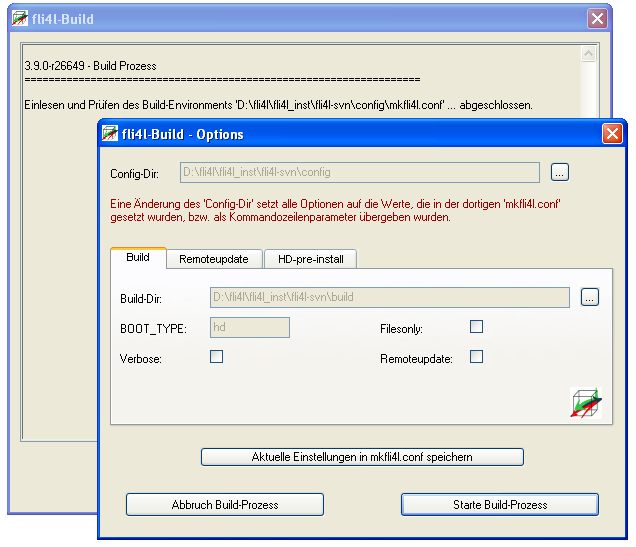
\includegraphics[width=\columnwidth]{win_build_build}
  \caption{Einstellungen}
  \label{fig:win_build_build}
  \end{figure}

  In diesem Dialog werden die Einstellungen für die Archiv/Bootmedienerstellung
  festgelegt:
  \begin{itemize}
    \item Build-Dir~-- Verzeichnis für die Archive/CD-Images/...
    \item \var{BOOT\_TYPE}~-- Anzeige des verwendeten/eingestellen \var{BOOT\_TYPE}~-- nicht änderbar
    \item Verbose~-- Aktivierung von zusätzlichen Ausgaben während der Erstellung
    \item Filesonly~-- es werden nur die Archive erstellt~-- kein bootmedium/kein Image
    \item Remoteupdate~-- Aktivierung des Remoteupdates per SCP
  \end{itemize}

  Mit der Schaltfläche \textbf{Aktuelle Einstellungen in mkfli4l.txt speichern}
  können die aktuell eingestellten Werte in der mkfli4l.txt gespeichert werden.

  \subsection{Konfigurationsdialog~-- Einstellungen für Remoteupdate}
  \begin{figure}[ht!]
  \centering
  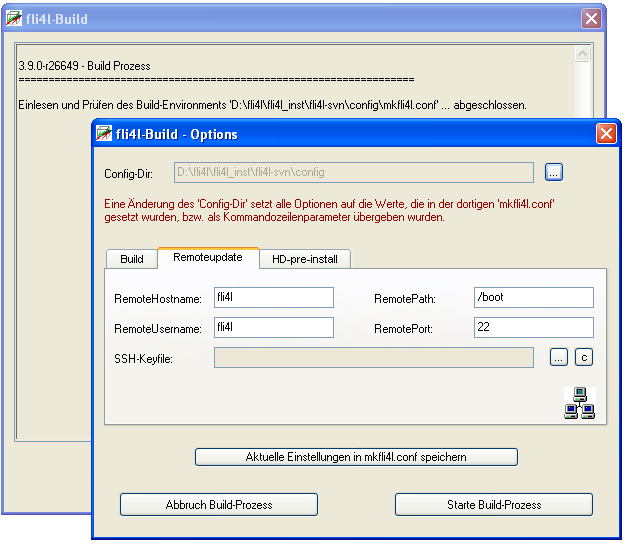
\includegraphics[width=\columnwidth]{win_build_remoteupdate}
  \caption{Einstellungen für Remoteupdate}
  \label{fig:win_build_remoteupdate}
  \end{figure}

  In diesem Dialog werden die Einstellungen für den Remoteupdate festgelegt:
  \begin{itemize}
    \item IP-Adresse oder Hostname
    \item Benutzername auf dem Remote-Host
    \item Remote-Pfad (default: /boot)
    \item Remote-Port (default: 22)
    \item zu verwendendes SSH-Keyfile (ppk-Format von Putty)
  \end{itemize}

  \subsection{Konfigurationsdialog~-- Einstellungen für HD-pre-install}
  \begin{figure}[ht!]
  \centering
  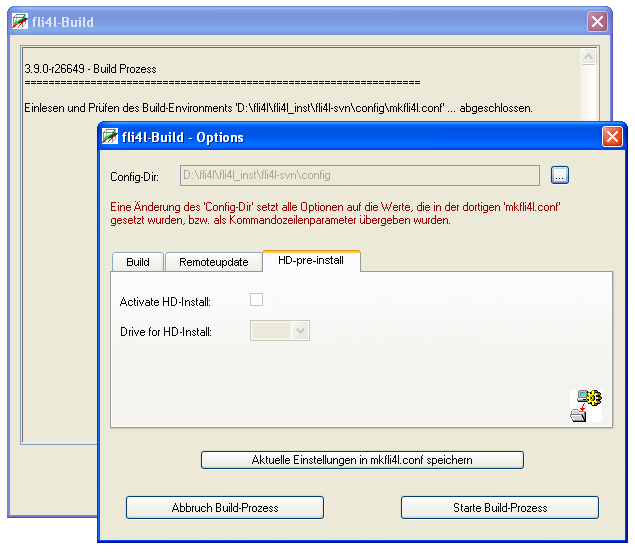
\includegraphics[width=\columnwidth]{win_build_hd_install}
  \caption{Einstellungen für HD-pre-install}
  \label{fig:win_build_hd_install}
  \end{figure}

   In diesem Dialog können die Optionen für den HD-pre-install auf einer
   entsprechend partitionierten und formatierten CompactFlash-Karte
   in einem USB-Reader eingestellt werden.

   Mögliche Optionen:
   \begin{itemize}
     \item HD-pre-install aktivieren
     \item Laufwerksbuchstabe der CF-Karte
  \end{itemize}

  Hinweis zur Partionierung und Formatierung der CF:
  Für eine HD-Installation nach TYP A (siehe dazu Paket HD) muss auf der CF eine
  primäre aktive und formatierte FAT-Partition vorhanden sein. Möchte man
  weiterhin auch eine Datenpartiton benutzen, wird zusätzlich eine Linux-Partition,
  die mit dem Dateisystem ext3 formatiert ist, sowie die Datei \texttt{hd.cfg} auf der
  FAT-Partiton benötigt (hierzu sollten unbedingt die Hinweise im Paket HD beachtet
  werden).

\marklabel{sec:mkfli4lconf}{
  \section{Steuerungsdatei mkfli4l.txt}}
  Seit fli4l-Version 2.1.9 existiert die Steuerungsdatei
  \texttt{$<$config$>$/mkfli4l.txt}. Durch sie werden z.B. vom Standard
  abweichende Verzeichnisse übergeben. Die Steuerungsdatei hat einen
  ähnlichen Aufbau wie die normalen fli4l Konfigurationsdateien.
  Alle Konfigurationsvariablen sind hier optional, d.h. sie müssen nicht
  in der Konfigurationsdatei vorkommen oder können als Kommentar gekennzeichnet
  werden.
  \begin{description}

  \config {BUILDDIR}{BUILDDIR}{BUILDDIR}

  Standardwert: `build'

  Legt fest, in welchem Verzeichnis die fli4l Dateien erzeugt werden sollen.
  Ist die Variable undefiniert, setzt mkfli4l unter Windows `build' relativ zum fli4l
  Wurzelverzeichnis ein und meint damit also das Verzeichnis
  \texttt{build} im fli4l Wurzelverzeichnis:
  \begin{verbatim}
    Pfad/fli4l-x.y.z/build
  \end{verbatim}
  \vspace{-2ex}
  Unter *nix setzt mkfli4l \texttt{$<$config$>$/build} ein und legt damit die
  generierten Dateien zusammen mit der Konfiguration ab.

  Die konfigurierten Pfade in \var{BUILDDIR} müssen der jeweiligen Logik von
  Windows oder *unix entsprechen. Werden relative Pfade gesetzt, wird der Pfad
  durch den Buildprozess passend zu Windows oder *unix konvertiert.

  \config {VERBOSE}{VERBOSE}{VERBOSE}

  Standardwert: \var{VERBOSE='no'}

  Mögliche Werte sind \var{'yes'} oder \var{'no'}. Steuert die \emph{Geschwätzigkeit}
  des Build Prozesses.

  \config {FILESONLY}{FILESONLY}{FILESONLY}

  Standardwert: \var{FILESONLY='no'}

  Mögliche Werte \var{'yes'} oder \var{'no'}. Hiermit kann das Erstellen eines
  Boot-Mediums abgeschaltet werden, es werden also nur die Dateien erzeugt~--

  \config {REMOTEUPDATE}{REMOTEUPDATE}{REMOTEUPDATE}

  Standardwert: \var{REMOTEUPDATE='no'}

  Mögliche Werte \var{'yes'} oder \var{'no'}. Aktiviert das automatische
  Übertragen der erstellten Dateien mittels SCP auf den Router. Dieses setzt
  ein installiertes Paket \jump{OPTSSHD}{SSHD} mit aktiviertem \texttt{scp}
  voraus.  Siehe dazu auch die folgenden Variablen.

  \config {REMOTEHOSTNAME}{REMOTEHOSTNAME}{REMOTEHOSTNAME}

  Standardwert: \var{REMOTEHOSTNAME=''}

  Gibt den Ziel-Hostnamen für den SCP Datentransfer an.
  Sollte kein Name angegeben sein, wird dieser der Variable
  \jump{HOSTNAME}{\var{HOSTNAME}} entnommen.

  \config {REMOTEUSERNAME}{REMOTEUSERNAME}{REMOTEUSERNAME}

  Standardwert: \var{REMOTEUSERNAME='fli4l'}

  Username für den SCP Datentransfer.

  \config {REMOTEPATHNAME}{REMOTEPATHNAME}{REMOTEPATHNAME}

  Standardwert: \var{REMOTEPATHNAME='/boot'}

  Ziel-Pfad für den SCP Datentransfer.

  \config {REMOTEPORT}{REMOTEPORT}{REMOTEPORT}

  Standardwert: \var{REMOTEPORT='22'}

  Zielport für den SCP Datentransfer.

  \config {SSHKEYFILE}{SSHKEYFILE}{SSHKEYFILE}

  Standardwert: \var{SSHKEYFILE=''}

  Hier kann man eine SSH-Keydatei für den SCP-Remoteupdate angeben.
  Es kann somit ein Update ohne Angabe eines Passwortes erfolgen.
  
  \config {REMOTEREMOUNT}{REMOTEREMOUNT}{REMOTEREMOUNT}
  
  Standardwert: \var{REMOTEREMOUNT='no'}
  
  Mögliche Werte \var{'yes'} oder \var{'no'}. Wird hier \var{'yes'}
  gesetzt, wird ein eventuell Readonly eingehängtes Bootdevice "/boot"
  für das Remoteupdate Readwrite gemountet um das Remoteupdate möglich
  zu machen. 

  \config {TFTPBOOTPATH}{TFTPBOOTPATH}{TFTPBOOTPATH}

  Pfad an dem das Netboot-Image abgelegt wird.

  \config {TFTPBOOTIMAGE}{TFTPBOOTIMAGE}{TFTPBOOTIMAGE}

  Name des Netboot-Images.

  \config {PXESUBDIR}{PXESUBDIR}{PXESUBDIR}

  Unterverzeichnis für die PXE-Dateien relativ zu TFTPBOOTPATH.


  \config {SQUEEZE\_SCRIPTS}{SQUEEZE\_SCRIPTS}{SQUEEZESCRIPTS}

   Aktiviert bzw. deaktiviert das Squeezen (Kommprimieren) von
   Skripten.
   Das Komprimieren eines Skripts mit Squeeze entfernt alle Kommentare und
   Zeileneinrückungen.
   Im Normalfall sollte hier immer der Standardwert \var{'yes'} benutzt werden.

  \config {MKFLI4L\_DEBUG\_OPTION}{MKFLI4L\_DEBUG\_OPTION}{MKFLI4LDEBUGOPTION}

   Es können zum Debuggen zusätzliche Optionen an das \jump{mkfli4l}{mkfli4l-Programm} übergeben
   werden.

  \end{description}

  \chapter{Anbindung von PCs im LAN}

  Für jeden Rechner im LAN ist einzustellen:

  \begin{enumerate}
  \item IP-Adresse (siehe \smalljump{sec:pc-lan-ip}{IP-Adresse})
  \item Name des Rechners plus Wunsch-Domain-Name
    (siehe \smalljump{sec:pc-lan-name}{Rechnername und Domain})
  \item Standard-Gateway (siehe \smalljump{sec:pc-lan-gateway}{Gateway})
  \item IP-Adresse des DNS-Servers (siehe \smalljump{sec:pc-lan-dns}{DNS-Server})
  \end{enumerate}

  \marklabel{sec:pc-lan-ip}{\section{IP-Adresse}}
  Die IP-Adresse muss im gleichen Netz wie die IP-Adresse des
  fli4l-Routers (auf Ethernet-Seite) liegen, also z.B. 192.168.6.2,
  wenn der fli4l die Adresse 192.168.6.1 hat.
  Kein Rechner darf die gleiche IP-Adresse haben, weshalb man am
  besten (nur) die letzte Zahl ändert. Auch ist darauf zu achten, dass
  man hier die gleiche IP-Adresse angibt, wie man es für diesen
  Rechner in der Datei config/base.txt angegeben hat.

  \marklabel{sec:pc-lan-name}{\section{Rechnername und Domain}}
  Der Name des Rechners ist dann z.B. ``mein-pc'', die Domain ``lan.fli4l''.

  \wichtig{Die im PC eingestellte Domain muss identisch mit der
  gewählten Domain im fli4l-Rechner sein, wenn man den fli4l-Router
  als DNS-Server verwenden will. Sonst kann es im Netz erhebliche
  Probleme geben.}

  Grund: Windows-Rechner suchen regelmäßig nach Rechnern mit dem Namen
  ihrer Arbeitsgruppte: WORKGROUP.meine-domain.fli4l. Ist dies nicht die in fli4l
  eingestellte Domain (hier: meine-domain.fli4l), wird fli4l
  versuchen, diese Anfrage durch Weiterleiten ins Internet zu
  beantworten \ldots

  Einzutragen ist die Domain in den TCP/IP Einstellungen des Rechners.

  \subsection{Windows 2000}

  Für Windows 2000 findet man das unter:

  \noindent Start \pfeil\\
  \hspace*{2ex}Einstellungen \pfeil\\
  \hspace*{4ex}Systemsteuerung \pfeil\\
  \hspace*{6ex}Netzwerk- und DFÜ-Verbindungen \pfeil\\
  \hspace*{8ex}LAN-Verbindung \pfeil\\
  \hspace*{10ex}Eigenschaften \pfeil\\
  \hspace*{12ex}Internetprotokoll (TCP/IP) \pfeil\\
  \hspace*{14ex}Eigenschaften \pfeil\\
  \hspace*{16ex}Erweitert\ldots \pfeil\\
  \hspace*{18ex}DNS \pfeil\\
  \hspace*{20ex}DNS-Suffix hinzufügen \pfeil\\

  ``lan.fli4l'' (bzw. die eingestellte domain) eingeben (ohne ``''!)
  \pfeil OK drücken.

\subsection{NT 4.0}

  Start \pfeil\\
  \hspace*{2ex}Einstellungen \pfeil\\
  \hspace*{4ex}Systemsteuerung  \pfeil\\
  \hspace*{6ex}Netzwerk \pfeil\\
  \hspace*{8ex}Protokolle \pfeil\\
  \hspace*{10ex}TCP/IP \pfeil\\
  \hspace*{12ex}Eigenschaften \pfeil\\
  \hspace*{14ex}DNS \pfeil\\
  \hspace{16ex}\begin{itemize}
  \item Hostname eintragen (eigener Rechnername)
  \item Domäne eintragen (wie in config/base.txt)
  \item IP-Adresse vom fli4l-Router hinzufügen
  \item DNS-Suffix hinzufügen (Domäne hinzufügen~-- siehe
    2 Zeilen höher)
  \end{itemize}

\subsection{Win95/98}

  Start \pfeil\\
  \hspace*{2ex}Einstellungen \pfeil\\
  \hspace*{4ex}Systemsteuerung \pfeil\\
  \hspace*{6ex}Netzwerk \pfeil\\
  \hspace*{8ex}Konfiguration \pfeil\\
  \hspace*{10ex}TCP/IP (jenes, das an die Netzwerkkarte zum Router\\
  \hspace*{10ex}angebunden ist) \pfeil\\
  \hspace*{12ex}Eigenschaften \pfeil\\
  \hspace*{14ex}DNS-Konfiguration:

  DNS aktivieren und bei ``Domäne:'' dann ``lan.fli4l'' eingeben (ohne ``''!).

\subsection{Windows XP}

  Für Windows XP findet man das unter:

  \noindent Start \pfeil\\
  \hspace*{2ex}Einstellungen \pfeil\\
  \hspace*{4ex}Systemsteuerung \pfeil\\
  \hspace*{6ex}Netzwerkverbindungen \pfeil\\
  \hspace*{8ex}LAN-Verbindung \pfeil\\
  \hspace*{10ex}Eigenschaften \pfeil\\
  \hspace*{12ex}Internetprotokoll (TCP/IP) \pfeil\\
  \hspace*{14ex}Eigenschaften \pfeil\\
  \hspace*{16ex}Erweitert\ldots \pfeil\\
  \hspace*{18ex}DNS \pfeil\\
  \hspace*{20ex}DNS-Suffix für diese Verbindung \pfeil\\

  ``lan.fli4l'' (bzw. die eingestellte domain) eingeben (ohne ``''!)
  \pfeil OK drücken.

\subsection{Windows 7}

  Für Windows 7 findet man das unter:

  \noindent Windows Button (ex. Start) \pfeil\\
  \hspace*{2ex}Systemsteuerung \pfeil\\
  \hspace*{4ex}Netzwerk und Internet \pfeil\\
  \hspace*{6ex}Netzwerk- und Freigabecenter \pfeil\\
  \hspace*{8ex}LAN-Verbindung \pfeil\\
  \hspace*{10ex}Eigenschaften \pfeil\\
  \hspace*{12ex}Internetprotokoll Version 4 (TCP/IPv4) \pfeil\\
  \hspace*{14ex}Eigenschaften \pfeil\\
  \hspace*{16ex}Erweitert\ldots \pfeil\\
  \hspace*{18ex}DNS \pfeil\\
  \hspace*{20ex}DNS-Suffix für diese Verbindung \pfeil\\

  ``lan.fli4l'' (bzw. die eingestellte domain) eingeben (ohne ``''!)
  \pfeil OK drücken.

\subsection{Windows 8}

  Für Windows 8 findet man das unter:

  \noindent Gleichzeitig Windows- und X-Taste drücken \pfeil\\
  \hspace*{2ex}Systemsteuerung \pfeil\\
  \hspace*{4ex}Netzwerk und Internet \pfeil\\
  \hspace*{6ex}Netzwerk- und Freigabecenter \pfeil\\
  \hspace*{8ex}Ihr Netzwerk wählen (Ehternet oder WLAN) \pfeil\\
  \hspace*{10ex}Eigenschaften \pfeil\\
  \hspace*{12ex}Internetprotokoll Version 4 (TCP/IPv4) \pfeil\\
  \hspace*{14ex}Eigenschaften \pfeil\\
  \hspace*{16ex}Erweitert\ldots \pfeil\\
  \hspace*{18ex}DNS \pfeil\\
  \hspace*{20ex}DNS-Suffix für diese Verbindung \pfeil\\

  ``lan.fli4l'' (bzw. die eingestellte domain) eingeben (ohne ``''!)
  \pfeil OK drücken.

  \marklabel{sec:pc-lan-gateway}{\section{Gateway}}
  Die Angabe des Standard-Gateways ist unbedingt erforderlich, denn
  ohne die Angabe der richtigen IP-Adresse an dieser Stelle
  funktioniert nichts.  Es muß hier die IP-Adresse des fli4l-Routers
  (auf Ethernet-Seite) angegeben werden, also z.B. 192.168.6.4
  entsprechend der IP-Adresse, die hier in der Datei config/base.txt
  für den fli4l-Router angegeben wurde.

  Es ist falsch, den fli4l-Router als Proxy in der Windows- oder
  Browser- Konfiguration einzutragen~-- außer man setzt ein Proxy auf
  dem fli4l-Router ein. Im Normalfall ist fli4l kein Proxy, daher
  bitte \emph{nicht} fli4l als Proxy angeben!

\marklabel{sec:pc-lan-dns}{\section{DNS-Server}}

  Als IP-Adresse des DNS-Servers gibt man nicht die Adresse des
  Provider-DNS-Servers an, sondern die des fli4l-Routers (Ethernet),
  da dieser nun selbst Anfragen beantworten kann bzw. diese bei
  Unkenntnis ins Internet weiterleitet.

  Mit der Konstruktion von fli4l als DNS-Server werden viele von den
  Windows-PCs ausgeführten Anfragen nicht ins Internet weitergeroutet,
  sondern werden direkt vom fli4l-Router beantwortet.

\marklabel{sec:pc-lan-misc}{\section{Verschiedenes}}

  Die Punkte 1 bis 4 brauchen bei konfiguriertem DHCP-Server nicht
  eingetragen zu werden, da dann der fli4l-Router die notwendigen Daten
  automatisch übermittelt.

  \textbf{Internetoptionen:} Bei Verbindungen muß ``keine Verbindung wählen'' ausgewählt sein.
  Bei Einstellungen für lokales Netzwerk(LAN): es darf hier NICHTS
  angegeben werden (es sei dann es wird \var{OPT\_\-P}roxy verwendet).
  Beides sind Standardeinstellungen, die im Normalfall nicht geändert
  werden müssen.

\marklabel{IMONDSCHNITTSTELLE}{
    \chapter{Client-/Server-Schnittstelle imon}
  }

  \marklabel{sec:imond}{
    \section{imon-Server imond}}

  imond ist ein netzwerkfähiges Server-Programm, welches bestimmte
  Anfragen beantwortet oder auch Kommandos zur Steuerung des Routers
  entgegennehmen kann.

  Ausserdem steuert imond das Least-Cost-Routing. Dazu verwendet er
  eine Konfigurationsdatei /etc/imond.conf, welche beim Booten
  automatisch aus den \var{ISDN\_\-CIRC\_\-x\_\-XXX}-Variablen der Datei
  config/isdn.txt und anderen über ein Shell-Script erzeugt wird.

  imond läuft permanent als Daemon und horcht gleichzeitig auf
  TCP/IP-Port 5000 und Device /dev/isdninfo.

  Folgende Kommandos sind über den TCP/IP-Port 5000 möglich:
  \begin{table}
    \textbf{Admin-Befehle}

    \vspace{1ex}
    \begin{tabular}{lp{9cm}}

      addlink ci-index              & Channel zum Circuit hinzufügen
                                      (Channel-Bundling) \\
      adjust-time seconds           & Ändert die Uhrzeit des Routers um die
                                      angegebenen Sekunden \\
      delete filename pw            & Löscht die Datei auf dem Router \\
      hup-timeout \#ci-index [value]& Anzeigen bzw. Setzen des HUP-Timeout für
                                      ISDN-Circuits \\
      removelink ci-index           & Zusätzlichen Channel wieder entfernen \\
      reset-telmond-log-file        & Löschen der telmond-Protokolldatei \\
      reset-imond-log-file          & Löschen der imond-Protokolldatei \\
      receive filename \#bytes pw   & Eine Datei auf den Router übertragen.
                                      Dazu quittiert imond den Befehl mit
                                      einem ACK (0x06). Danach wird die Datei
                                      in 1024er-Blöcken übertragen, die imond
                                      auch jeweils mit einem ACK bestätigt.
                                      Als letztes übermittelt imond noch ein
                                      OK. \\
      send filename pw              & Wenn das Passwort stimmt und die Datei
                                      existiert, liefert imond ein OK \#bytes.
                                      Anschliessend überträgt imond die Datei
                                      in 1024er Blöcken, die jeweils mit
                                      einem ACK (0x06) bestätigt werden
                                      müssen. Als letztes liefert imond noch
                                      ein OK. \\
      support pw                    & Liefert den Status/Konfiguration vom
                                      Router \\
      sync                          & Synchronisiert den Cache von gemounteten
                                      Laufwerken \\
    \end{tabular}
  \end{table}


  \begin{table}
    \textbf{Admin- oder User-Befehle}

    \vspace{1ex}
    \begin{tabular}{lp{9cm}}

      dial                      &    Wählt den Provider an
                                     (Default-Route-Circuit) \\
      dialmode [auto|manual|off]&    Liefert bzw. setzt den Dialmode \\
      disable                   &    Hängt ein und setzt dialmode auf ``off''
                                      \\
      enable                    &    Setzt dialmode auf ``auto'' \\
      halt                      &    Fährt den Router sauber herunter \\
      hangup [\#channel-id]     &    Hängt ein \\
      poweroff                  &    Fährt den Router herunter und schaltet ab \\
      reboot                    &    Reboot vom i4l-Router! \\
      route [ci-index]          &    Setzen Default-Route auf Circuit X
                                     (0=automatisch) \\
    \end{tabular}
  \end{table}


  \begin{table}
    \textbf{User-Befehle}

    \vspace{1ex}
    \begin{tabular}{lp{9cm}}
      channels                  & Ausgabe Anzahl der verfügbaren ISDN-Kanäle\\
      charge \#channel-id       & Ausgabe der Online-Kosten für einen
                                  Channel\\
      chargetime \#channel-id   & Online-Zeit unter Berücksichtigung des
                                  Taktes\\
      circuit [ci-index]        & Ausgabe eines Circuit-Namens\\
      circuits                  & Ausgabe Anzahl der Default-Route-Circuits\\
      cpu                       & Liefert die Auslastung der CPU in Prozent\\
      date                      & Ausgabe Datum/Uhrzeit\\
      device ci-index           & Liefert das Device des Circuits\\
      driverid \#channel-id     & Ausgabe Driver-Id für Channel X\\
      help                      & Ausgabe Hilfe\\
      inout \#channel-id        & Ausgabe der Richtung (incoming/outgoing)\\
      imond-log-file            & Ausgabe imond-Protokolldatei\\
      ip \#channel-id           & Ausgabe der IP\\
      is-allowed command        & Ausgabe, ob Befehl konfiguriert/gültig
                                  ist\newline
                                  Mögliche Befehle:
                                    dial|dialmode|route|reboot|
                                    imond-log|telmond-log|mgetty-log \\
      is-enabled                & Ausgabe, ob dialmode auf off (0) oder auto
                                  (1)\\
      links ci-index            & Ausgabe Anzahl momentaner Channel 0, 1 oder
                                  2, 0 heisst: Kein Channel-Bundling möglich\\
      log-dir imond|telmond|mgetty& Liefert das Logverzeichnis\\
      mgetty-log-file           & Ausgabe mgetty-Protokolldatei\\
      online-time \#channel-id  & Ausgabe Online-Zeit der akt. Verbindung in
                                  hh:mm:ss\\
      pass [password]           & Abfrage, ob Password nötig bzw. Password-
                                  Eingabe\newline
                                  1 Userpassword gesetzt\newline
                                  2 Adminpassword gesetzt\newline
                                  4 imond befindet sich im Admin-Modus\\
      phone \#channel-id        & Ausgabe Telefonnummer/Name des ``Gegners''\\
      pppoe                     & Liefert die Anzahl der pppoe-Devices (also 0
                                  oder 1)\\
      quantity \#channel-id     & Liefert die übertragenen Datenmengen (in
                                  Byte)\\
      quit                      & Beenden der Verbindung zu imond\\
      rate \#channel-id         & Ausgabe Übertragungsraten (incoming/outgoing
                                  in B/sec)\\
      status \#channel-id       & Ausgabe Status für Channel X\\
      telmond-log-file          & Ausgabe telmond-Protokolldatei\\
      time \#channel-id         & Ausgabe Summe Online-Zeiten, Format
                                  hh:mm:ss\\
      timetable [ci-index]      & Ausgabe der Zeittabelle für LC-Routing\\
      uptime                    & Ausgabe der Uptime des Routers in Sekunden\\
      usage \#channel-id        & Ausgabe Art der Verbindung, mögliche
                                  Antworten: Fax, Voice, Net, Modem, Raw\\
      version                   & Ausgabe der Protokoll- und
                                  Programm-Version\\
    \end{tabular}
  \end{table}


  Der TCP/IP-Port 5000 ist nur vom maskierten LAN aus erreichbar.
  Standardmäßig wird ein Zugriff von aussen über die
  Firewall-Konfiguration abgeblockt.

  Imond unterstützt zwei Benutzerebenen: den User- und den
  Admin-Modus.  Für beide Ebenen kann ein Passwort gesetzt werden
  mittels \var{IMOND\_\-PASS} bzw.  \var{IMOND\_ADMIN\_\-PASS}. Dadurch
  werden die imon-Clients von imond gezwungen, eine Password-Abfrage
  durchzuführen und anschließend das Password an imond zu übertragen.
  Solange dieses Password nicht übermittelt wurde, nimmt imond nur die
  beiden Kommandos ``pass'' und ``quit'' entgegen. Alle anderen werden
  mit einem Fehler zurückgewiesen.

  Möchte man das weiter einschränken, z.B. den Zugriff nur von nur
  einem PC erlauben, muss die Firewall-Konfiguration angepasst werden.

  Die Befehle

\begin{example}
\begin{verbatim}
         enable/disable/dialmode   dial/hangup   route   reboot/halt
\end{verbatim}
\end{example}

  können durch die Konfigurationsvariablen \var{IMOND\_\-XXX} global ein- oder
  abgeschaltet werden (s. Kapitel ``Konfiguration'').

  Mit einem Unix/Linux-Rechner (oder einem Windows-Rechner in der DOS-Box)
  kann man das Ganze leicht ausprobieren:

  Nach Eingabe von

\begin{example}
\begin{verbatim}
        telnet fli4l 5000        \# oder entsprechender Name des fli4l-Routers
\end{verbatim}
\end{example}

  kann man direkt die oben aufgeführten Kommandos eingeben und sich
  die Ausgabe anschauen.

  Zum Beispiel bekommt man mit ``help'' die Hilfe angezeigt, mit
  ``quit'' wird die Verbindung zum imond abgebaut.

\marklabel{sec:leastcostrouting}{
  \subsection{Least-Cost-Routing~-- Funktionsweise}
  }

  imond konstruiert aus der Konfigurationsdatei /etc/imond.conf
  (welche wiederum beim Booten aus den Konfigurationsvariablen
  \var{ISDN\_\-CIRC\_\-x\_\-TIMES} usw.  erstellt wird), eine zeitabhängige
  Tabelle (Time-Table). Diese umfasst eine komplette Kalenderwoche im
  1-Stunden-Raster (168 Stunden = 168 Bytes). Die Tabelle setzt sich
  jedoch lediglich aus Circuits zusammen, für die eine Default-Route
  definert ist.

  Mit dem imond-Kommando ``timetable'' kann man sich diese Tabelle
  anschauen.

  Hier ein Beispiel:

  Nehmen wir an, dass 3 Circuits definiert wurden, nämlich:

\begin{example}
\begin{verbatim}
        CIRCUIT_1_NAME='Addcom'
        CIRCUIT_2_NAME='AOL'
        CIRCUIT_3_NAME='Firma'
\end{verbatim}
\end{example}

  wobei lediglich die ersten beiden Circuits mit Default-Routen belegt
  sind, also die enstprechenden Variablen ISDN\_CIRC\_x\_ROUTE den
  Wert `0.0.0.0' haben.

  Wenn die dazugehörigen Variablen \var{ISDN\_\-CIRC\_\-x\_\-TIMES} folgendermaßen
  aussehen:

\begin{example}
\begin{verbatim}
        ISDN_CIRC_1_TIMES='Mo-Fr:09-18:0.0388:N Mo-Fr:18-09:0.0248:Y
                      Sa-Su:00-24:0.0248:Y'

        ISDN_CIRC_2_TIMES='Mo-Fr:09-18:0.019:Y Mo-Fr:18-09:0.049:N
                      Sa-Su:09-18:0.019:N Sa-Su:18-09:0.049:N'

        ISDN_CIRC_3_TIMES='Mo-Fr:09-18:0.08:N Mo-Fr:18-09:0.03:N
                      Sa-Su:00-24:0.03:N'
\end{verbatim}
\end{example}

  dann wird daraus folgende Datei /etc/imond.conf:

\begin{example}
\begin{verbatim}
        #day  hour  device  defroute  phone        name        charge  ch-int
        Mo-Fr 09-18 ippp0   no        010280192306 Addcom      0.0388   60
        Mo-Fr 18-09 ippp0   yes       010280192306 Addcom      0.0248   60
        Sa-Su 00-24 ippp0   yes       010280192306 Addcom      0.0248   60
        Mo-Fr 09-18 ippp1   yes       019160       AOL  0.019   180
        Mo-Fr 18-09 ippp1   no        019160       AOL  0.049   180
        Sa-Su 09-18 ippp1   no        019160       AOL  0.019   180
        Sa-Su 18-09 ippp1   no        019160       AOL  0.049   180
        Mo-Fr 09-18 isdn2   no        0221xxxxxxx  Firma       0.08     90
        Mo-Fr 18-09 isdn2   no        0221xxxxxxx  Firma       0.03     90
        Sa-Su 00-24 isdn2   no        0221xxxxxxx  Firma       0.03     90
\end{verbatim}
\end{example}

  imond erstellt dann im Speicher folgende Time-Table~-- hier die Ausgabe
  über das imond-Kommando ``timetable'':

\begin{example}
\begin{verbatim}
         0  1  2  3  4  5  6  7  8  9 10 11 12 13 14 15 16 17 18 19 20 21 22 23
     --------------------------------------------------------------------------
     Su  3  3  3  3  3  3  3  3  3  3  3  3  3  3  3  3  3  3  3  3  3  3  3  3
     Mo  2  2  2  2  2  2  2  2  2  4  4  4  4  4  4  4  4  4  2  2  2  2  2  2
     Tu  2  2  2  2  2  2  2  2  2  4  4  4  4  4  4  4  4  4  2  2  2  2  2  2
     We  2  2  2  2  2  2  2  2  2  4  4  4  4  4  4  4  4  4  2  2  2  2  2  2
     Th  2  2  2  2  2  2  2  2  2  4  4  4  4  4  4  4  4  4  2  2  2  2  2  2
     Fr  2  2  2  2  2  2  2  2  2  4  4  4  4  4  4  4  4  4  2  2  2  2  2  2
     Sa  3  3  3  3  3  3  3  3  3  3  3  3  3  3  3  3  3  3  3  3  3  3  3  3

     No.  Name                   DefRoute  Device  Ch/Min   ChInt
      1   Addcom                   no      ippp0   0.0388     60
      2   Addcom                   yes     ippp0   0.0248     60
      3   Addcom                   yes     ippp0   0.0248     60
      4   AOL               yes     ippp1   0.0190    180
      5   AOL               no      ippp1   0.0490    180
      6   AOL               no      ippp1   0.0190    180
      7   AOL               no      ippp1   0.0490    180
      8   Firma                    no      isdn2   0.0800     90
      9   Firma                    no      isdn2   0.0300     90
     10   Firma                    no      isdn2   0.0300     90
\end{verbatim}
\end{example}

  Für den Circuit 1 (Addcom) sind also drei Zeitbereiche (1-3)
  eingetragen, für Circuit 2 (AOL) vier Zeitbereiche (4-7) und
  für den letzen drei Zeitbereiche (8-10).

  In der Time-Table werden jeweils die Indices ausgegeben, welche für
  die jeweilige Stunde gültig sind. Hier tauchen lediglich die Indices
  2-4 auf, da alle anderen keine LC-Default-Routen sind.

  Sieht man in der Tabelle irgendwo Nullen, gibt es Lücken in den
  \var{ISDN\_\-CIRC\_\-X\_\-TIMES}-Werten. Dann existiert zu diesen Zeiten keine
  Default-Route, Internet-Zugang abgeknipst!

  Beim Programmstart ermittelt imond zunächst den Wochentag und die
  aktuelle Stunde. Anschließend wird dann über die Time-Table der
  Index ermittelt und damit dann auch der entsprechende Circuit. Auf
  diesen wird dann die Default-Route gesetzt.

  Bei Zustandsänderungen der Channels, z.B. Wechsel von online
  nach offline~-- jedoch spätestens nach 1 Minute~-- geht das Spiel von
  neuem los: Zeit ermitteln, Lookup in Tabelle, Default-Route-Circuit
  ermitteln.

  Ändert sich der aktuell verwendete Circuit, z.B. montags um 18:00
  Uhr, wird die alte Default-Route gelöscht, eine vielleicht
  bestehende Verbindung beendet (sorry\ldots) und anschließend die
  Default-Route auf den neuen Circuit gesetzt. Dies kann von imond bis
  zu 60 Sekunden später bemerkt werden, also wird spätestens um
  18:00:59 umgeschaltet.

  Bei Circuits, die keine Default-Route belegen, ändert sich überhaupt
  nichts. Hier wird der Inhalt von \var{ISDN\_\-CIRC\_\-x\_\-TIMES} lediglich zur
  Berechnung der Telefonkosten verwendet. Diese können dann relevant
  sein, wenn man über den Client imonc das LC-Routing temporär
  ausschaltet und einen Circuit manuell wählt.

  Man kann sich jedoch auch die Tabellen für andere
  Zeitbereich-Indices (im Beispiel von 1 bis 10) anschauen, auch die
  der ``Non-LC-Default-Route-Circuits''.

  Kommando:

\begin{example}
\begin{verbatim}
                    timetable index
\end{verbatim}
\end{example}

  Beispiel:

\begin{example}
\begin{verbatim}
                    telnet fli4l 5000
                    timetable 5
                    quit
\end{verbatim}
\end{example}

  Die Ausgabe sieht dann so aus:

\begin{example}
\begin{verbatim}
         0  1  2  3  4  5  6  7  8  9 10 11 12 13 14 15 16 17 18 19 20 21 22 23
     --------------------------------------------------------------------------
     Su  0  0  0  0  0  0  0  0  0  0  0  0  0  0  0  0  0  0  0  0  0  0  0  0
     Mo  5  5  5  5  5  5  5  5  5  0  0  0  0  0  0  0  0  0  5  5  5  5  5  5
     Tu  5  5  5  5  5  5  5  5  5  0  0  0  0  0  0  0  0  0  5  5  5  5  5  5
     We  5  5  5  5  5  5  5  5  5  0  0  0  0  0  0  0  0  0  5  5  5  5  5  5
     Th  5  5  5  5  5  5  5  5  5  0  0  0  0  0  0  0  0  0  5  5  5  5  5  5
     Fr  5  5  5  5  5  5  5  5  5  0  0  0  0  0  0  0  0  0  5  5  5  5  5  5
     Sa  0  0  0  0  0  0  0  0  0  0  0  0  0  0  0  0  0  0  0  0  0  0  0  0

     No.  Name                   DefRoute  Device  Ch/Min   ChInt
      5   AOL               no      ippp1   0.0490    180
\end{verbatim}
\end{example}

  Alles klar?

  Mit dem imond-Kommando ``route'' kann das LC-Routing ein- und
  ausgeschaltet werden. Bei Angabe eines positiven Circuit-Indices
  (1\ldots N) wird die Default-Route auf den angegebenen Circuit
  gelegt. Ist der Index 0, wird das LC-Routing wieder aktiviert und
  der Circuit automatisch ausgewählt.


  \subsection{Zur Berechnung der Onlinekosten}

  Das ganze Modell zur Berechnung der Onlinekosten funktioniert nur
  korrekt, wenn der Zeittakt für einen Circuit (Variable
  \var{ISDN\_\-CIRC\_\-x\_\-CHARGEINT}) über die ganze Woche konstant ist. Dies
  ist im Normalfall bei Internet-Providern die Regel. Wählt man sich
  jedoch über die Telekom (ich meine nicht T-Online!) z.B. in sein
  Firmennetz ein, gilt das als ganz normales Telefongespräch. Und da
  wechselt ab 18:00 der Takt von 90 Sekunden auf 4 Minuten (Stand Juni
  00). Deshalb ist die Definition von

\begin{example}
\begin{verbatim}
        ISDN_CIRC_3_CHARGEINT='90'
        ISDN_CIRC_3_TIMES='Mo-Fr:09-18:0.08:N Mo-Fr:18-09:0.03:N Sa-Su:00-24:0.03:N'
\end{verbatim}
\end{example}

  eigentlich nicht ganz korrekt. Es sind zwar abends umgerechnet auf
  die Minute 3 Pfennig (4 Minuten kosten 12 Telekom-Pfennige), jedoch
  ist der Takt falsch. Deshalb können bei der Kostenanzeige
  Differenzen zu den tatsächlichen Zahlen auftreten.

  Hier ist ein Tipp, wie verschieden lange Taktzeiten dennoch richtig
  berücksichtigt werden können (auch wichtig für
  \var{ISDN\_\-CIRC\_\-x\_\-CHARGEINT}): Man definiert einfach 2 Circuits,
  einen für tagsüber mit \var{ISDN\_\-CIRC\_\-1\_\-CHARGEINT}=`90' und den
  anderen mit \var{ISDN\_\-CIRC\_\-2\_\-CHARGEINT}=`240'.
  Natürlich muss man dann auch noch \var{ISDN\_\-CIRC\_\-x\_\-TIMES}
  entsprechend wählen, damit tagsüber Circuit 1 und abends Circuit 2
  verwendet wird.

  Wie gesagt: Bei Nutzung von Verbindungen zu Internet-Providern gibt
  es das Problem nicht, weil dort der Zeittakt immer konstant ist und
  lediglich die Kosten pro Minute wechseln (oder gibt es sowas doch???
  Ich traue T-* alles zu :-).

  % Last Update: $Id$
  \marklabel{sec:winimonc}{
    \section{Windows-Client imonc.exe}}

  \subsection{Einleitung}

  Das Gespann imond auf dem Router und imonc auf dem Client beherrschen
  zwei Benutzermodi: den User- und den Adminmodus. Im Adminmodus sind alle
  Steuerelemente aktiviert. Im Usermodus steuern die Variablen 
  \jump{IMONDENABLE}{\var{IMOND\_ENABLE}}, \jump{IMONDDIAL}{\var{IMOND\_DIAL}}, 
  \jump{IMONDROUTE}{\var{IMOND\_ROUTE}} und \jump{IMONDREBOOT}{\var{IMOND\_REBOOT}} ob die
  jeweiligen Funktionen im Usermodus zur Verfügung stehen. Sind alle diese 
  Variablen auf `no' gesetzt, bedeutet dies für die Überblick-Seite, dass alle 
  Buttons bis auf den Exit- und den Admin-Mode-Button deaktiviert sind. Die 
  Entscheidung, ob der User- oder Admin-Modus benutzt wird, wird anhand des 
  übermittelten Passwortes getroffen. Über den Button Admin-Mode, der sich in 
  der Statusleiste befindet, kann jederzeit unter Eingabe des Admin-Passwortes 
  vom User- zum Admin-Modus gewechselt werden. Um wieder zurück zu wechseln, 
  muss imonc beendet und neu gestartet werden.

  Sobald imonc gestartet ist, wird ein zusätzliches Tray-Icon angezeigt, welches 
  den Verbindgungsstatus der vorhandenen Kanäle anzeigt.

  Die Farben bedeuten:
  \begin{description}
    \item[Rot]: Offline
    \item[Gelb]: Es wird gerade eine Verbindung aufgebaut
    \item[Hellgrün]: Online und Traffic auf dem Kanal
    \item[Dunkelgrün]: Online und so gut wie kein Traffic auf dem Kanal
  \end{description}
  
  \noindent Ein etwas vom Windows-Standard abweichendes Verhalten zeigt imonc, wenn der 
  Minimieren-Button in der Titelleiste angeclickt wird. Daraufhin minimiert sich 
  imonc in den Systemtray und es bleibt nur noch das Tray-Icon neben der Uhr 
  übrig. Ein Doppelklick mit der linken Maustaste auf das Tray-Symbol holt das 
  imonc-Fenster wieder in den Vordergrund. Mit der rechten Maustaste besteht 
  auch die Möglichkeit über das Kontextmenü, die wichtigsten imonc-Kommandos 
  direkt auszuwählen, ohne imonc wieder auf den Bildschirm zu holen.

  Viele Eigenschaften (darunter auch alle Spaltenbreiten der StringGrids) 
  speichert imonc in der Registry, damit imonc so an die eigenen Bedürfnisse 
  angepasst werden kann. Imonc speichert die Informationen in dem 
  Registry-Schlüssel HKCU{\textbackslash}Software{\textbackslash}fli4l.

  Bestehen trotz sorgfältigen Lesens der Dokumentation noch Probleme in Bezug 
  auf imonc oder auch des Routers selber, die man z.B. in der Newsgroup posten 
  möchte, ist es sinnvoll, auf der Über-Seite des imonc den Punkt SystemInfo 
  auszuwählen und dort den Punkt Support Infos. Daraufhin wird das 
  Router-Passwort abgefragt (nicht das imond-Passwort!). Imonc erstellt dann 
  eine Datei fli4lsup.txt, welche alle wichtigen Informationen bezüglich des 
  Routers und imonc beinhaltet. Diese Datei kann auf explizite Nachfrage in die 
  Newsgroup gepostet werden, so dass deutlich bessere Chancen auf rasche Hilfe
  bestehen.

  Nähere Details betreffend der Entwicklung des Windows-Clients imonc findet man 
  auf der Homepage vom Windows ImonC-Seiten \altlink{http://www.imonc.de/}. Hier 
  kann man sehen, welche neuen Features und Bug-Fixes in der nächsten Version 
  von imonc enthalten sein werden. Ausserdem gibt es dort den neusten imonc, 
  wenn dieser nicht schon in der fli4l-Distribution enthalten ist.

  \subsection{Startparameter}

  ImonC benötigt den Namen oder die IP-Adresse des fli4l-Routers. Standardmäßig 
  versucht das Programm, eine Verbindung mit dem Rechner ``fli4l'' herzustellen. 
  Wenn dieser im DNS korrekt eingetragen ist, sollte es also direkt 
  funktionieren. Ansonsten kann man in der Verknüpfung folgende Parameter 
  übergeben:

  \begin{itemize}
    \item /Server:IP oder Hostname des Routers (Kurzform: /S:IP oder Hostname)
    \item /Password:Passwort (Kurzform: /P:Password)
    \item /log Die Logging-Option zum Protokollieren der Kommunikation zwischen 
      imonc und imond. Ist diese Option eingeschaltet, wird beim Beenden von 
      imonc eine Datei imonc.log geschrieben. Diese Datei beinhaltet die gesamte 
      Kommunikation zwischen Router und Client und wird darum sehr groß. Deshalb 
      sollte dieser Startparameter nur gesetzt werden, wenn Probleme bestehen.
    \item /iport:Portnummer Die Portnummer auf die imond lauscht. Default: 5000
    \item /tport:Portnummer Port auf dem telmond lauscht. Default: 5001
    \item /rc:''Command'' Das hier angegebene Kommando wird ohne weitere 
      Überprüfung an den Router übertragen und anschliessend imonc beendet. 
      Sollen mehrere Kommandos gleichzeitig ausgeführt werden, müssen diese 
      durch Semikolons getrennt werden. Damit es funktioniert, muss ein 
      gesetztes imond-Passwort mit übergeben werden, da keine Abfrage des
      Passwortes erfolgt. Die möglichen Kommandos sind beim imond dokumentiert,
      siehe Kapitel 8.1. Zusätzlich zu den dort aufgeführten Befehlen gibt es
      noch den Befehl timesync. Dieser bewirkt, dass die Uhrzeit des Clients
      mit der des Routers synchronisiert wird. Der Befehl dialtimesync wird
      nicht mehr unterstützt da er sich als \glqq{}dial; timesync\grqq{} schreiben lässt.
    \item /d:''fli4l-Directory'' Hiermit kann das fli4l-Directory per 
      Startparameter übergeben werden. Interessant wenn man mit mehreren
      fli4l-Versionen herumspielt
    \item /wait Wenn der Hostname nicht aufgelöst werden kann, beendet sich 
      imonc nicht mehr~-- erneuter Verbindungsaufbau durch Doppelclick auf das 
      TrayIcon
    \item /nostartcheck Dieser schaltet die Überprüfung ab, ob imonc bereits 
      läuft. Nur sinnvoll, wenn mehrere, unterschiedliche fli4l-Router in einem 
      Netz überwacht werden sollen. Bei weiteren Instanzen werden die 
      eingebauten Syslog- und \mbox{E-Mail}-Funktionalitäten deaktiviert.
  \end{itemize}

  Usage (einzutragen in der Verknüpfung):

\begin{example}
\begin{verbatim}
X:\...imonc.exe [/Server:Host] [/Password:Passwort] [/iport:Portnummer]
            [/log] [/tport:Portnummer] [/rc:"Command"]
\end{verbatim}
\end{example}

  Beispiel mit IP-Adresse:

\begin{example}
\begin{verbatim}
        C:\wintools\imonc /Server:192.168.6.4
\end{verbatim}
\end{example}

  oder mit Namen und Passwort:

\begin{example}
\begin{verbatim}
        C:\wintools\imonc /S:fli4l /P:geheim
\end{verbatim}
\end{example}

  oder mit Namen, Passwort und Routerkommando:

\begin{example}
\begin{verbatim}
        C:\wintools\imonc /S:fli4l /P:geheim /rc:"dialmode manual"
\end{verbatim}
\end{example}

  \subsection{Seite Überblick}

  Der Windows-Client fragt einige imond-Informationen über die bestehenden 
  Verbindungen ab und bereitet sie im Anzeigefenster auf. Neben generellen 
  Statusinformationen wie Uptime des Router oder auch der Uhrzeit sowohl lokal 
  wie auch vom Router selber, werden für jede bestehende Verbindung die 
  folgenden Informationen angezeigt:
  
  \begin{tabular}{lp{9cm}}
    Status             &Verbindungsaufbau/Online/Offline\\
    Name               &Telefonnummer des Gegners oder Circuit-Name\\
    Richtung           &Zeigt an, ob es sich um eine eingehende oder ausgehende
    Verbindung handelt\\
    IP                 &Die IP, die man zugewiesen bekommen hat\\
    IBytes             &Empfangene Bytes\\
    OBytes             &Gesendete Bytes\\
    Online-Zeit        &Aktuelle Online-Zeit\\
    Zeit               &Summe aller Online-Zeiten\\
    KZeit              &Summe Online-Zeiten unter Berücksichtigung des Zeittaktes\\
    Kosten             &Berechnete Kosten\\
  \end{tabular}

  \medskip

  Die Daten werden standardmäßig alle 2 Sekunden aktualisiert. Im Kontextmenü
  dieser Übersicht besteht die Möglichkeit für jeden vorhandenen Kanal, mit dem 
  der Router gerade online ist, sowohl die zugewiesene IP in die Zwischenablage 
  zu kopieren, als auch den Kanal gezielt auflegen zu können. Letzteres ist für 
  den Fall interessant, dass mehrere unterschiedliche Verbindungen bestehen, 
  z.B. eine um im Internet zu surfen und eine andere zur Firma, und gezielt eine 
  dieser Verbindungen getrennt werden soll.

  Ist zusätzlich auf dem fli4l-Router der telmond-Prozess aktiv, kann imonc 
  zusätzlich Informationen über eingehende Telefonanrufe (nämlich anrufende und 
  angerufene MSN) anzeigen. Der letzte eingegangene Telefonanruf wird oberhalb 
  der Buttons angezeigt.   Ein Protokoll der eingegangenen Telefonanrufe erhält 
  man durch Anzeige der Seite Anrufe.

  Mit den sechs Buttons im imonc können folgende Kommandos angewählt werden:

  \begin{tabular}{clp{9cm}}
    Button & Beschriftung & Funktion \\
    1& Verbinden/Trennen  & Wählen/Einhängen\\
    2& Add link/Rem link  & Kanäle bündeln: ja/nein~-- dieses Feature steht nur
                            im Admin-Mode zur Verfügung\\
    3& Reboot             & fli4l neu booten!\\
    4& PowerOff           & fli4l sauber runterfahren und anschliessend
                            ausschalten\\
    5& Halt               & fli4l sauber runterfahren, um ihn anschliessend
                            sicher ausschalten zu können\\
    6& Beenden            & Client beenden\\
  \end{tabular}

  \medskip

  \noindent Die ersten fünf Kommandos können in der Konfigurationsdatei des fli4l-Routers
  config/base.txt für den User-Modus einzeln ein- und ausgeschaltet werden. Im 
  Admin-Modus sind immer alle aktiviert.
  Die Auswahl Dialmode steuert das Wahlverhalten des Routers:

  \begin{tabular}{lp{9cm}}
    Auto    & Der Router baut automatisch eine Verbindung auf dem entsprechenden
              Circuit auf, wenn eine Anfrage aus dem lokalen Netz eintrifft.\\
    Manuell & Der Benutzer muss selber die Verbindung aufbauen.\\
    Aus     & Es ist weder manuell noch automatisch möglich, eine
              Verbindung aufzubauen. Der Dial-Button ist dann deaktiviert.\\
  \end{tabular}

  \medskip

  \noindent Bleibt noch anzumerken, dass fli4l standardmäßig selbständig rauswählt, wenn
  man mit seinem Rechner in's Internet will. Man muss also eigentlich nie den 
  Verbinden-Button drücken \ldots

  Es besteht auch die Möglichkeit, den Default-Route-Circuit manuell zu 
  wechseln, also das automatische LCR-Routing ein- und auszuschalten. Dafür ist 
  in der Windows-Version von imonc die Auswahlliste ``Default Route'' 
  vorgesehen. Ausserdem kann man die Hangup-TimeOut-Zeit jetzt auch über imonc 
  direkt konfigurieren. Dazu dient der Button Config neben der Default Route. 
  Dort werden alle konfigurierten Circuits des Routers angezeigt. Der Wert in 
  der Spalte Hup-timeout kann für ISDN-Circuits direkt im StringGrid editiert 
  werden (funktioniert bis dato noch nicht für DSL).

  Einen Überblick über das LCR-Routing findet man auf der Seite Admin/TimeTable. 
  Dort sieht man, welchen Circuit imond zu welcher Zeit automatisch auswählt.


  \subsection{Config-Dialog}

  Der Konfigurationsbereich ist über den Button Config in der Statuszeile 
  erreichbar. Das aufgehende Fenster ist dann in die folgenden Bereiche 
  unterteilt:

  \begin{itemize}
  \item Der Bereich Allgemein:
    \begin{itemize}
    \item Aktualisierungsintervall: Hier wird eingestellt, wie oft die Seite
      Überblick aktualisiert werden soll.
    \item Zeit beim Programmstart synchronisieren: Übernimmt beim Starten des
      Client die Zeit und das Datum des Routers als lokale Zeit. Diese Funktion 
      kann auch manuell mit dem Button Synchronisieren auf der Überblicks-Seite 
      aufgerufen werden.
    \item Minimiert starten: Startet das Programm direkt minimiert, man sieht 
      nur das Icon neben der Uhr.
    \item Zusammen mit Windows starten: Hier kann man angeben, ob der Client 
      direkt beim Starten von Windows mit gestartet werden soll. In dem Feld 
      Parameter kann man die nötigen Start-Parameter angeben.
    \item News von fli4l.de abholen: Sollen die News, die auf der fli4l-Homepage 
      in der News-Sektion angezeigt werden, auch vom imonc geholt und angezeigt 
      werden? Die Schlagzeilen werden dann in der Statusbar angezeigt. Ausserdem 
      wird dann eine neue Seite News angezeigt, in der die kompletten Meldungen 
      angezeigt werden.
    \item Logdatei für Verbindungen: Den Dateinamen, den man hier angeben kann, 
      wird dazu benutzt, die Verbindungs-Liste unter diesem Namen lokal auf dem 
      Rechner abzuspeichern.
    \item TimeOut für Router zum antworten: Wie lange soll auf eine Antwort der 
      Routers gewartet werden, bevor angenommen wird, dass die Verbindung nicht 
      mehr besteht.
    \item Sprache: Hier kann die Sprache des imoncs ausgewählt werden.
    \item Router Befehle bestätigen: Ist dieses Feature aktiviert, müssen alle 
      Router"=beeinflussenden Kommandos, wie zum Beispiel Reboot, Hangup \ldots
      generell bestätigt werden.
    \item Auflegen auch bei Traffic: Soll kein Hinweis erfolgen, wenn die 
      Verbindung beendet wird und noch Traffic auf der Leitung ist.
    \item Automatisch Verbindung zum Router aufbauen: Soll, wenn die Verbindung 
      zum Router unterbrochen wird (z.B. durch einen Neustart des Routers),
      automatisch probiert werden, die Verbindung wieder herzustellen.
    \item Fenster in System Tray minimieren: Soll imonc beim Clicken auf den 
      Beenden-Button in der Titelleiste sich in den System-Tray neben der Uhr
      minimieren anstatt zu beenden.
    \end{itemize}

  \item Der Unterbereich Proxy:
    Hier kann ein Proxy für die http-Anfragen des imoncs definiert werden. 
    Dieser wird dann zur Zeit für das Holen der News benutzt.
    \begin{itemize}
    \item Proxy-Unterstützung für Http-Anfragen aktivieren: Soll ein Proxy 
      benutzt werden
          \begin{itemize}
            \item Adresse: Die Adresse des Proxy-Servers
            \item Port: Die Portnummer des Proxy-Server (default: 8080)
          \end{itemize}
    \end{itemize}
    
  \item Der Unterbereich TrayIcon:
  	Hier können die Farben des TrayIcons neben der Uhr an die eigene Bedürfnisse
  	angepasst werden. Weiterhin kann ausgewählt werden, dass der aktuelle
  	Dialmode als farblicher Hintergrund des TrayIcons dargestellt wird.

  \item Der Bereich Anrufe: Die Position des Call Notification-Fensters wird in 
    der Registry gespeichert, so dass man sich das Fenster an die Position 
    schieben kann, wo man es haben möchte. Es erscheint anschliessend immer 
    wieder an dieser Stelle.
    \begin{itemize}
      \item Aktualisierung: Hier kann ausgewählt werden, wie imonc über neue
        Anrufe informiert wird. Es gibt drei verschiedene Möglichkeiten. Diese
        erste besteht darin, regelmäßig den telmond-Dienst auf dem Router 
        abzufragen. Eine weitere Möglichkeit besteht in der Auswertung der 
        Syslog-Meldungen. Diese Variante ist der ersten vorzuziehen~-- dazu muss
        natürlich der Syslog-Client des imonc aktiviert sein. Wird imonc mit 
        einem routenden eisfair eingesetzt, bietet sich noch die Möglichkeit das
        Capi2Text-Paket zur Anrufsignalisierung zu benutzen.
      \item Führende Null wegen Telefonanlage löschen: Telefonanlage setzen 
        manchmal eine zusätzliche Null vor die Rufnummer des Anrufer. Diese kann 
        mit dieser Option unterdrückt werden.
      \item Eigene Vorwahl: Hier kann die eigene Vorwahl hinterlegt werden. Wann 
        dann ein Anruf mit gleichen Vorwahl eintrifft, wird die gesendete 
        Vorwahl ausgeblendet.
      \item Telefonbuch: Hier kann die Datei angegeben werden, in der das lokale 
        Telefonbuch zur Auflösung von Telefonnummer gespeichert wird. Existiert 
        die Datei nicht, wird sie vom Programm angelegt.
      \item Logdatei: Der Dateinamen, den man hier angeben kann, wird dazu 
        benutzt, die Calls-Liste unter diesem Namen lokal auf dem Rechner zu 
        speichern. Dieser Menüpunkt ist nur sichtbar, wenn die Config-Variable 
        \var{TELMOND\_\-LOG} auf `yes' gesetzt ist, dieses gilt auch für die 
        eigentliche Anruf-Liste.
      \item Externes Suchprogramm benutzen: In diesem Bereich kann ein Programm
        angegeben werden, dass aufgerufen wird, wenn eine Telefonnummer mittels 
        des lokalen Telefonbuches nicht aufgelöst werden kann. Nähere Infos 
        sollten den entsprechenden Programmen beiliegen. Bis jetzt gibt es eine 
        Anbindung an die Telefonbuch-CD KlickTel sowie von Marcel Wappler eine 
        Anbindung an die Palm-Datenbank.
    \end{itemize}

  \item Der Unterbereich Call Notification: 
    Hier kann das bestimmt werden, ob ein Hinweis auf eingehende Telefonanrufe
    angezeigt werden soll und wie dieser sich optisch präsentiert.
    \begin{itemize}
      \item Call Notification aktivieren: Bestimmt, ob Anrufe signalisiert
        werden sollen.
      \item Call Notification anzeigen: Soll bei eingehenden Anrufen ein
        Hinweisfenster mit den Infos: angerufene MSN, Rufnummer des Anrufers und 
        Datum/Uhrzeit erscheinen? Dafür ist es nötig, dass in der Datei 
        config/isdn.txt die Variable \var{OPT\_\-TELMOND} auf `yes' gesetzt 
        wird.
        \begin{itemize}
          \item Unterdrücken, wenn keine Nummer übertragen wurde: Soll Die 
            Call Notification nicht angezeigt werden, wenn keine Rufnummer 
            übertragen wurde.
          \item Anzeigendauer: Diese Angabe beeinflußt die Dauer, wie lange das 
            Call Noti\-fication-Fenster geöffnet bleiben soll. Die Angabe von 
            ``0'' an dieser Stelle bewirkt, dass das Fenster nicht automatisch 
            geschlossen wird.
          \item Fontsize: Hiermit wird die Schriftgröße bestimmt. Dieses hat 
            einen Einfluss auf die Größe des Fenster, da die notwendige Größe 
            des Fenster anhand der tatsächlichen Größe der Mitteilung berechnet 
            wird.
          \item Farbe: Hiermit kann die Schriftfarbe ausgewählt werden. Ich 
            selber benutzte die Farbe rot, damit ich es auch direkt wahrnehme.
      \end{itemize}
    \end{itemize}
    

  \item Der Unterbereich Phonebook: Die Seite Phonebook beinhaltet das
    Telefonbuch, welches zur Rufnummerauflösung der anrufenden Nummer
    als auch der eigenen MSN benutzt wird. Die Seite wird auch
    angezeigt, wenn die Konfigurationsvariable \var{TELMOND\_\-LOG} auf `no'
    gesetzt ist, da die Rufnummerauflösung auch für die Anzeige des
    letzten Anrufes auf der Summary-Seite benutzt wird. Alternativ
    kann statt dem Telefonbuch auf dem Router auch eine lokale Datei
    ausgewählt werden.

    Der Aufbau der Eintrag sieht wie folgt aus:

\begin{example}
\begin{verbatim}
  # Format:
  # Telefonnummer=anzuzeigender Name[, Wavefilename]
  # 0241123456789=Testuser
  00=unbekannt
  508402=Fax
  0241606*=Elsa AG Aachen
\end{verbatim}
\end{example}

    Dabei sind die ersten drei Zeilen Kommentare. Die vierte Zeile
    bewirkt, dass, wenn keine Rufnummer übermittelt wird,
    ``unbekannt'' angezeigt wird. In der fünften Zeile wird der MSN
    508402 der Name ``Fax'' zugeordnet. Ansonsten ist das Format immer
    Telefonnummer=Name, der stattdessen angezeigt werden soll. In der
    sechsten Zeile ist noch die Möglichkeit demonstriert, eine
    Sammelrufnummer zu definieren. Damit wird erreicht, dass für alle
    Nebenstellen von 0241606 der Name angezeigt wird. Zu beachten
    hierbei ist, dass der erste Eintrag im Telefonbuch, welcher auf
    den Anruf passt, genommen wird. Optional kann auch noch ein
    Wave-Datei angegeben werden, die abgespielt wird, wenn ein
    Telefonanruf von dieser Rufnummer eingeht.

    Ab der Version 1.5.2 besteht jetzt auch die Möglichkeit auf der
    Seite Names das lokale Telefonbuch mit dem auf dem Router
    abgespeicherten (in /etc/phonebook) zu synchronisieren und
    umgekehrt. Dabei werden nicht nur einfach die Dateien ersetzt,
    sondern es werden die noch fehlende Einträge hinzugefügt. Gibt es
    eine Telefonnummer in beiden Telefonbüchern mit unterschiedlichen
    Namen, wird nachgefragt, welcher Eintrag genommen werden soll. Für
    die Synchronisierung des Telefonbuches auf dem Router ist noch
    anzumerken, dass dieses nur in der Ramdisk verändert wird, d.h.
    dass nach einem Reboot sämtliche Änderungen verloren gehen.

  \item Der Bereich Sound: Die Wave-Dateien, die hier angegeben werden, werden 
    abgespielt, wenn das jeweilige Ereignis eingetreten ist.
    \begin{itemize}
      \item \mbox{E-Mail}: Wenn der \mbox{E-Mail}-Checker auf einem angegebenen POP3-Server neue 
        \mbox{E-Mails} vorfindet, wird die angegebene Wave-Datei abgespielt.
      \item \mbox{E-Mail}-Error: Wenn ein Fehler beim Abrufen der \mbox{E-Mails} auftritt, wird 
        diese Wave-Datei abgespielt.
      \item Verbindung verloren: Wenn die Verbindung zum Router nicht mehr
        vorhanden ist (z.B. wenn der Router von einem anderen Client gerade neu 
        gebootet wird), wird diese Wave-Datei abgespielt. Wenn die Option 
        ``Automatic Reconnect to router'' nicht aktiviert ist, erscheint 
        ausserdem eine MessageBox, die nachfragt, ob versucht werden soll, eine 
        neue Verbindung zum Router aufzubauen.
      \item Verbindungsmeldung: Wenn der Router eine Verbindung zum Internet
        aufgebaut hat, wird diese Wave-Datei abgespielt.
      \item Verbingsabbau: Wenn der Router die Verbindung zum Internet wieder 
        abgebaut hat, wird diese Wave-Datei abgespielt.
      \item Anrufmeldung: Wenn die Call Notification aktiviert ist und ein neuer 
        Anruf eingeht, wird die angegebene Wave-Datei abgespielt.
      \item Fax Notification: Die hier angegebene Wave-Datei wird nach dem 
        Empfang neuer Faxe abgespielt.
    \end{itemize}

  \item Der Bereich \mbox{E-Mails}
    \begin{itemize}
      \item Accounts: Dieser Bereich dient dazu, die vorhandenen
        POP3-Accounts zu konfigurieren.
      \item \mbox{E-Mail}-Check aktivieren: Soll der \mbox{E-Mail}-Checker automatisch nach neuen
        \mbox{E-Mails} suchen
        \begin{itemize}
          \item Check jede x Min: Hiermit wird angegeben, wie oft der 
            \mbox{E-Mail}-Checker automatisch nach neuen \mbox{E-Mails} suchen soll. Achtung: ein 
            zu kurzes Intervall kann dazu führen, dass der Router komplett 
            online bleibt! Dies ist der Fall, wenn das Intervall kleiner ist als 
            der Hangup-Timeout des verwendeten Circuits.
          \item TimeOut x Sec: Wie lange soll auf einen einen POP3-Server 
            gewartet werden, bis er antwortet. Der Wert ``0'' bedeutet, dass 
            kein TimeOut gesetzt wird.
          \item Auch wenn Router offline: Hiermit wird erreicht, dass der Router 
            sich selbstständig einwählt, um nach \mbox{E-Mails} zu sehen. Nachdem alle 
            POP3-Konton nach \mbox{E-Mails} überprüft worden sind, wird die Verbindung 
            wieder getrennt. Um dieses Feature nutzen zu können, muss Dialmode 
            auf `auto' stehen. Achtung: Dadurch entstehen zusätzliche Kosten, 
            wenn nicht gerade eine Flatrate benutzt wird!
          \item Zu benutzender Circuit: Hiermit wird angegeben, welcher Circuit
            zur Einwahl beim \mbox{E-Mail}-Checken benutzt werden soll.
          \item Anschliessend online bleiben: Soll direkt nach dem \mbox{E-Mail}-Check 
            direkt die Verbindung getrennt werden oder eine 
            Verbindungstrennung durch das Hangup-timeout realisiert werden.
          \item \mbox{E-Mail}-Header laden: Sollen auch die \mbox{E-Mail}-Header geladen oder 
            nur die Anzahl der vorhandenen \mbox{E-Mails} abgefragt werden? Das Laden 
            der \mbox{E-Mail}-Header ist Voraussetzung, wenn man \mbox{E-Mails} direkt auf dem
            Server löschen möchte.
         \item Notify only new \mbox{E-Mails}: Sollen nur neue \mbox{E-Mails} akustisch und mit 
           dem Tray-Icon gemeldet werden
         \item \mbox{E-Mail}-Client starten: Soll der angegebene \mbox{E-Mail}-Client 
           automatisch gestartet werden, wenn neue \mbox{E-Mails} vorhanden sind.
         \item \mbox{E-Mail}-Client: Hier wird der zu startende \mbox{E-Mail}-Client angegeben.
         \item Param: Hier kann man zusätzliche Parameter angeben, die beim 
           Start des \mbox{E-Mail}-Clients übergeben werden sollen. Wenn Outlook als 
           \mbox{E-Mail}-Client benutzt wird (nicht Outlook Express), sollte /recyle als 
           Parameter eingetragen werden, damit eine bereits geöffnete Instanz 
           von Outlook beim Eintreffen von neuen \mbox{E-Mails} benutzt wird.
      \end{itemize}
    \end{itemize}

  \item Der Bereich Admin
    \begin{itemize}
      \item root-Passwort: Hier sollte das Router-Passwort (in config/base.txt 
        unter \verb+PASSWORD+ eingetragen) eingetragen werden, damit z.B. das 
        Portforwarding lokal bearbeitet und wieder auf dem Router hinterlegt 
        werden kann.
      \item Dateien auf dem Router, die angezeigt werden sollen: Alle hier 
        angegebenen Dateien, die sich auf dem Router befinden, können einfach 
        per Maus-Click auf der Seite Admin/Dateien angezeigt werden. Somit kann 
        man sich auf einfache Weise die Logfiles des Routers direkt im imonc 
        anzeigen lassen.
      \item Konfigdateien bearbeiten: Hier kann ausgewählt werden, ob die
        Konfigdateien alle im Editor geöffnet werden sollen (dies kann, wenn 
        TXT-Dateien noch mit einem einfachen Editor verknüpft sind, dazu führen, 
        dass sehr viele Instanzen des Editors geöffnet werden). Alternativ kann 
        auch einfach nur das Verzeichnis geöffnet werden, so dass die 
        Möglichkeit besteht, nur die Dateien auszuwählen, die bearbeitet werden 
        sollen.
      \item DynEisfaiLog: Wenn ein Account bei DynEisfair vorhanden ist, kann 
        man hier seine Zugangsdaten eintragen und sich dann ein Log der 
        Aktualisierung des Dienstes auf der Seite Admin/DynEisfairLog anschauen.     
    \end{itemize}

  \item Der Bereich LaunchList dient dazu, die Launchliste zu konfigurieren. 
    Diese wird nach einem erfolgreichen Connect ausgeführt, wenn die Option 
    ``Activate Launchlist'' aktiviert ist.
    \begin{itemize}
      \item Programme: Alle hier eingetragenen Programme werden automatisch 
        gestartet, sobald der Router eine Verbindung aufgebaut hat und die
        Launchliste aktiviert ist.
      \item LaunchList aktivieren: Soll die Launchliste beim erfolgreichen
        Verbindungsaufbau ausgeführt werden?
    \end{itemize}

  \item Der Bereich Traffic dient dazu, dass TrafficInfo-Fenster den eigenen 
    Bedürfnissen anzupassen. Von einem User habe ich den Hinweis bekommen, dass 
    es mit älteren DirectX-Versionen offenbar Darstellungsfehler gibt.
    \begin{itemize}
      \item Separates Traffic-Info-Fenster anzeigen: Soll eine grafische 
        Kanalauslastung in einem separaten Fenster angezeigt werden? In dem 
        Kontextmenü des Fensters kann man festlegen, ob das Fenster das 
        Attribut StayOnTop bekommen soll. Dieses bewirkt, dass sich das Fenster 
        immer über allen anderen Fenstern plaziert. Auch dieser Wert wird in der 
        Registry abgespeichert und steht somit auch nach einem erneuten 
        Programmstart wieder zur Verfügung.
      \item Titelleiste anzeigen: Soll die Titelleiste des Traffic-Info-Fensters 
        angezeigt werden? In der Titelzeile wird angezeigt, mit welchem Circuit 
        der Router gerade online ist.
        \begin{itemize}
          \item CPU-Auslastung in Titelleiste: Soll auch die CPU-Auslastung in
            der Titelzeile angezeigt werden?
          \item Online-Zeit in Titelleiste: Soll die Onlinezeit des Kanals auch 
            in der Titelzeile angezeigt werden?
        \end{itemize}
      \item Semi-transparentes Fenster: Soll das Fenster transparent dargestellt 
        werden? Diese Funktion steht nur unter Windows 2000 und Windows XP zur 
        Verfügung.
      \item Farben: Hier werden die Farben für das TrafficInfo-Fenster 
        definiert. Zu Berücksichtigen ist dabei, dass der DSL-Kanal und der 
        erste ISDN-Kanal die selben Farbwerte zugewiesen bekommen.
      \item Limits: Hier können die max. Übertragungswerte für DSL eingestellt 
        werden~-- Upload und Download.
    \end{itemize}

  \item Der Bereich Syslog dient dazu, die Anzeige der Syslog-Meldungen zu 
    konfigurieren.
    \begin{itemize}
      \item Syslog-Client aktivieren: Sollen Syslog-Meldungen im imonc angezeigt 
        werden? Diese Option sollte ausgeschaltet sein, wenn ein externer 
        Syslog-Client, wie zum Beispiel Kiwi's Syslog Client, benutzt wird.
      \item Alle Meldungen ab Stufe anzeigen: Ab welcher Prioritätsstufe sollen 
        die Syslog-Meldungen angezeigt werden? Es ist sinnvoll am Anfang mit der 
        Stufe Debug anzufangen, um damit festzustellen, welche Meldungen einen 
        interessieren. Anschliessend kann hier dann die entsprechende Stufe 
        eingetragen werden.
      \item Syslog-Meldungen in einer Datei speichern: Sollen die angezeigten
        Syslog-Meldungen in einer Datei gespeichert werden? In der Groupbox 
        können dann die Meldungen ausgewählt werden, die in der Datei geloggt 
        werden sollen. Für den Dateinamen sind folgende Platzhalter eingefügt 
        worden:
        \begin{description}
          \item[\%y]~-- wird durch das aktuelle Jahr ersetzt
          \item[\%m]~-- wird durch den aktuellen Monat ersetzt
          \item[\%d]~-- wird durch den aktuellen Tag ersetzt
        \end{description}
      \item Portnamen anzeigen: Sollen statt den Portnummern deren Bedeutungen
        angezeigt werden?
      \item Firewall-Meldungen auch im User-Modus anzeigen: Hiermit wird
        festgelegt, dass Firewall-Meldungen auch im User-Modus angezeigt werden
        sollen.
    \end{itemize}

  \item Der Bereich Fax dient dazu, die Faxanzeige vom imonc zu konfigurieren. 
    Damit dieser Punkt angezeigt wird, muss mgetty bzw. faxrcv auf dem Router 
    installiert sein (zu finden als OPT-Pakete auf der fli4l-Homepage).
    \begin{itemize}
      \item Logdatei für Faxe: Den Dateinamen, den man hier angeben kann, wird 
        dazu benutzt, die Fax-Liste unter diesem Namen lokal auf dem Rechner 
        abzuspeichern.
      \item Lokales Verzeichnis: Um die Faxe anzeigen zu können, müssen sie
        lokal gespeichert werden. Dieses kann hier eingestellt werden.
      \item Aktualisierung: Es gibt zwei verschiedene Möglichkeiten, wie imonc
        mitbekommt, dass ein neues Fax eingegangen ist. Entweder wertet imonc
        die entsprechenden Syslogmeldungen aus (dazu muss natürlich der 
        Syslog-Client im imonc aktiviert sein) oder er schaut regelmäßig selber
        in der Logdatei nach. Die erste Variante ist zu bevorzugen. Falls die
        zweite Variante genutzt wird, kann man noch angeben, wieoft die
        Faxübersichtsseite aktualisiert werden soll. Dabei ist zu beachten, dass 
        dieser Wert keine Angabe in Sekunden ist, sondern noch mit der Angabe 
        von Allgemein/Aktualisierungsintervall multipliziert wird. 
    \end{itemize}

  \item Der Bereich Grids dient dazu die Grids (Tabellen) im imonc an die 
    eigenen Bedürfnisse anzupassen. Einerseits kann für jedes Grid angegeben 
    werden, welche Spalten angezeigt werden sollen, andererseits gibt es die 
    Möglichkeit für die Grids im Bereich Anrufe, Verbindungen und Faxe 
    anzugeben, von wann ab die Infos angezeigt werden sollen.
  \end{itemize}

  \subsection{Seite Anrufe}

  Die Seite Calls wird nur angezeigt, wenn die Konfigurationsvariable
  \var{TELMOND\_\-LOG} auf `yes' eingestellt ist, denn sonst wird kein
  Anruf-Log geführt. Auf dieser Seite werden alle abgespeicherten
  Telefonanrufe angezeigt, die eingegangen sind, während der Router
  eingeschaltet war. Dabei kann umgeschaltet werden zwischen der
  Ansicht der lokal gespeicherten Anrufe oder nur der auf dem Router
  gespeicherten Anrufe. Wird bei der Anzeige der auf dem Router
  gespeicherten Anrufe der Zurücksetzen-Button gedrückt, wird das Logfile auf
  dem Router gelöscht.

  In der Anruf-Übersicht kann mit der rechten Maustaste auf der
  Rufnummer oder der eigenen MSN diese ins Telefonbuch übernommen
  werden, um der Rufnummer bzw. MSN dort einen Namen zuzuweisen, der
  dann stattdessen angezeigt wird.


  \subsection{Seite Verbindungen}

  Neu ist ab der Version 1.4 die Anzeige der vom Router aufgebauten
  Verbindungen zum Internet. Diese befindet auf der Seite Connections.
  Somit hat man einen guten Überblick, wie sich der Router bei der
  automatischen Einwahl ins Internet verhält. Damit diese Seite
  angezeigt werden kann, muss in der Datei config/base.txt die
  Variable \var{IMOND\_\-LOG} auf `YES' gesetzt werden.

  Genauso wie bei der Anruf-Übersicht kann auch hier zwischen den
  lokal gespeicherten und auf dem Router gespeicherten Verbindungen
  umgeschaltet werden.  In der Ansicht der auf dem Router
  gespeicherten Verbindungen bewirkt ein Drücken des Zurücksetzen-Buttons,
  dass das Logfile auf dem Router gelöscht wird.

  Angezeigt werden pro Verbindung
  \begin{itemize}
  \item Provider
  \item Startdatum und -zeit
  \item Enddatum und -zeit
  \item Onlinezeit
  \item Abrechnungszeit
  \item entstandene Kosten
  \item empfangene Zeichen
  \item gesendete Zeichen
  \end{itemize}

  \subsection{Seite Fax}

  Damit die Seite Faxe angezeigt wird, muss auf dem Router entweder das
  \var{OPT\_\-MGETTY} von Michael Heimbach oder \var{OPT\_\-MGETTY} von Felix Eckhofer
  installiert werden. Diese gibt es auf der fli4l-Homepage unter
  OPT-Pakete. Auf dieser Seite werden dann alle eingegangenen Faxe
  aufgelistet. Das Kontextmenü der Übersicht bietet mehrere Möglichkeiten,
  diese stehen allerdings nur im Admin-Modus zur Verfügung:

  \begin{itemize}
  \item Es kann ein Fax angezeigt werden. Dazu muss unter
    Admin/Remoteupdate der Pfad für das fli4l-Verzeichnis korrekt
    gesetzt werden, da die Faxe auf dem Router in gepackter Form
    vorliegen und somit gzip aus dem fli4l-Paket benötigt wird.
    Alternativ kann gzip.exe und win32gnu.dll auch ins
    imonc-Verzeichnis kopiert werden. Kann gzip.exe nicht an einer der
    beiden Stellen gefunden werden, wird stattdessen der Webserver des
    Routers probiert zu öffnen (direkt mit dem Aufruf des richtigen
    CGIs).
  \item Ein einzelnes Fax kann gelöscht werden. Dabei wird das Fax
    sowohl lokal als auch auf dem Router gelöscht (sowohl die
    eigentliche Faxdatei, als auch der Eintrag in den Logdateien).
  \item Sämtliche auf dem Router befindlichen Faxe löschen. Damit
    werden die Faxe und die Logdatei auf dem Router gelöscht. Die Faxe
    werden nicht aus der lokalen Logdatei gelöscht.
  \end{itemize}
  Genauso wie bei der Anruf-Übersicht kann auch hier zwischen den
  lokal gespeicherten und auf dem Router gespeicherten Faxen
  umgeschaltet werden.


  \subsection{Seite E-Mail}

  Diese Seite wird nur angezeigt, wenn im Config-Dialog mindestens ein
  aktiviertes POP3-\mbox{E-Mail}-Konto eingerichtet worden ist.

  Die Seite \mbox{E-Mail} dürfte sich eigentlich selber erklären. Hiermit wird
  der mittlerweile eingebaute \mbox{E-Mail}-Checker beobachtet. Ist die Option
  ``Check even if the router is offline'' nicht aktiviert, überprüft
  der \mbox{E-Mail}-Checker alle \mbox{E-Mail}-Konten nach \mbox{E-Mails}, sobald der Router
  online ist und anschließend im eingestellt Intervall. Ist die
  genannte Option aktiviert, überprüft der \mbox{E-Mail}-Checker im
  eingestellten Intervall. Ist der Router gerade online, wird die
  bestehende Verbindung benutzt. Ist er nicht online, wird eine
  Verbindung selbständig mit dem ausgewählten Circuit hergestellt,
  die, sobald alle \mbox{E-Mail}-Konten abgearbeitet sind, wieder getrennt
  wird. Damit man diese Option nutzen kann, muss Dialmode auf ``auto''
  stehen.

  Sind \mbox{E-Mails} auf dem POP3-Server vorhanden, wird entweder automatisch
  der eingestellte \mbox{E-Mail}-Client gestartet oder ein neues Symbol im
  Tray neben der Uhr angezeigt, welches als Hint die Anzahl der \mbox{E-Mails}
  auf jedem Server liefert. Ein Doppelclick startet dann den
  eingestellten \mbox{E-Mail}-Client. Ist ein Fehler bei einem der
  \mbox{E-Mail}-Konten aufgetreten, erscheint einerseits ein Hinweis in der
  \mbox{E-Mail}-History, andererseits wird das \mbox{E-Mail}-TrayIcon angezeigt,
  welches dadurch gekennzeichnet ist, dass die obere rechte Ecke rot
  gefärbt ist.

  In der \mbox{E-Mail}-Übersicht kann man mit dem Kontextmenü Mails direkt auf
  dem Server löschen, ohne sie vorher komplett downloaden zu müssen.
  Dies geschieht, indem mit der rechten Maustaste das Kontextmenü
  angezeigt wird. Dabei sollte eine Zelle der entsprechenden Zeile
  markiert sein, wo die zu löschende \mbox{E-Mail} eingetragen ist. Im
  Kontextmenü wählt man den einzige Punkt Delete MailMessage aus.


  \subsection{Admin}

  Dieser Abschnitt steht nur zur Verfügung, wenn sich imonc im
  Admin-Modus befindet.

  Der erste Punkt lieferte eine Übersicht über die verwendeten
  Circuits~-- sprich Internetprovider~-- die der Router automatisch per
  LCR auswählt. Ein Doppelclick auf einen Provider in der
  Providerübersicht zeigt an, für welche Zeiträume der Circuit in
  config/base.txt definiert worden ist.

  Der zweite Punkt dort ist die Möglichkeit ein Fernupdate auf dem
  Router einzuspielen. Dabei kann ausgewählt werden, welche fünf
  Programmpakete (Kernel, Rootfilesystem, Opt-Datei, rc.cfg und syslinux.cfg) auf 
  den Router kopiert werden sollen. Damit man das Update einspielen kann,
  muss man zuerst mal das fli4l-Verzeichnis angeben, damit imonc
  weiss, woher es die nötigen Dateien nehmen soll. Ausserdem muss
  angegeben werden, in welchem Unterverzeichnis die Konfigurationsdateien liegen 
  (standardmäßig config), um die Opt-Datei, rc.cfg und syslinux.cfg 
  jeweils neu zu erzeugen. Es ist ratsam, einen Reboot nach dem Einspielen des
  Updates durchführen, damit die Änderungen auch direkt wirksam
  werden.  Wird während des Updates nach einem Passwort nachgefragt,
  ist das Passwort gemeint, welches in config/base.txt unter PASSWORD
  eingetragen ist.

  Um die Beschränkung des Port-Forwarding zu umgehen, dass ein Port nur
  an genau einen Client-Rechner gebunden ist, besteht jetzt die Möglichkeit,
  die Konfiguration auf dem Router zu editieren. Damit die Änderungen aktiv
  werden, muss die Verbindung neu hergestellt werden. Da die Datei nur in
  der Ramdisk ersetzt wird, bleiben die Änderungen nur bis zum nächsten
  Neustart des Routers erhalten. Um die Änderungen dauerhaft zu speichern,
  muss ein neues Opt-File auf dem Router installiert werden mit einer
  geeignet angepassten base.txt aus dem Config-Verzeichnis.

  Der vierte Punkt auf der Admin-Seite~-- Dateien~-- dient dazu,
  Konfigurations- und Logdateien des Routers einfach per Maus-Click
  anzuzeigen. Die Auswahlliste wird über den Punkt Config/Admin und
  dort ``files on router to view'' konfiguriert.  Anschliessend kann
  einfach über die ComboBox auf dieser Seite ausgewählt werden, welche
  Datei angezeigt werden soll.

  Der fünfte Punkt ist die Seite DynEisfairLog, sie erscheint nur wenn im 
  Config-Dialog unter Admin die Zugangsdaten des DynEisfair-Accounts eingetragen
  worden sind. Ist dies geschehen, wird auf dieser Seite Log des Dienstes 
  angezeigt.
  
  Als letzten Punkt gibt es noch die Seite Hosts. Hier werden alle in der Datei
  /etc/hosts eingetragenen Rechner angezeigt. Weiterhin wird probiert jeden 
  dieser dort eingetragenen Rechner anzupingen und das Ergebnis davon wird 
  ebenfalls angezeigt. Somit kann man schnell rausbekommen, welche dieser 
  Rechner eingeschaltet sind. 

  \subsection{Seiten Fehler, Syslog und Firewall}

  Die Seiten Fehler, Syslog und Firewall werden nur angezeigt, wenn in
  den entsprechenden Logs Einträge vorhanden sind. Die Einträge der
  Seiten Syslog und Firewall werden nur angezeigt, wenn man im
  Admin-Modus ist.

  Auf der Seite Fehler werden sämtliche imonc/imond-spezifischen Fehler
  festgehalten. Wenn Probleme bestehen, kann unter Umständen ein Blick
  auf diese Seite die Ursache der Probleme anzeigen.

  Auf der Seite Syslog werden die ankommende Syslog-Meldungen
  angezeigt, bis auf die Meldungen der Firewall. Diese werden auf der
  eigenen Seite Firewall dargestellt. Damit dies funktioniert, muss
  die Variable \var{OPT\_\-SYSLOGD} in der Konfigurationsdatei config/base.txt
  auf `yes' gesetzt werden. Ausserdem muss die Variable \var{SYSLOGD\_\-DEST}
  auf die IP des Clients gesetzt werden (genau:
  \var{SYSLOGD\_\-DEST}='@100.100.100.100~-- wobei die IP natürlich an die IP
  des Clients angepasst werden muss).  Angezeigt wird neben der
  eigentlichen Syslog-Meldung auch Datum, Uhrzeit, IP des Senders und die
  Prioritätsstufe.

  Damit die Firewall-Meldungen bei den ganzen Syslog-Meldungen nicht
  untergehen, werden diese auf der separaten Seite Firewall angezeigt.
  Damit die Firewall- Meldungen angezeigt werden können, muss
  zusätzlich in der Datei config/base.txt die Konfigurationsvariable
  \var{OPT\_\-KLOGD} auf `yes' gesetzt werden.

  \subsection{Seite News}

  Auf dieser Seite werden, vorausgesetzt die Option ist im Config-Bereich des
  Imonc aktiviert, die News, welche auf der fli4l-Homepage angezeigt werden,
  auch direkt im Imonc angezeigt werden. Dazu wird mittels des http-Protokolls 
  die URL http://www.fli4l.de/german/news.xml abgerufen. Neben den News werden
  mittlerweile auch die fünf aktuellsten Opt-Pakete angezeigt. Dazu wird 
  die URL http://www.fli4l.de/german/imonc\_opt\_show.php abgefragt. Außerdem
  wird in der Statusleiste vom Imonc die Überschriften der News alternierend
  angezeigt.


  \marklabel{sec:imonc}{
    \section{Unix/Linux-Client imonc}}

  Für Linux gibt es mittlerweile 2 Versionen: eine textbasierte
  (imonc) und eine mit graphischer Oberfläche (ximonc). Den Source zu
  ximonc findet man im Verzeichnis src. Die Dokumentation für ximonc
  wird erst in der 1.5-Final-Version zur Verfügung stehen. Ein
  erfahrener Linux-User sollte aber mit den Sources keine Probleme
  haben.

  Beschränken wir uns daher hier zunächst auf die textbasierte Version
  von imonc: Dieses ist ein curses-basiertes Programm, hat also keine
  graphische Oberfläche. Der Source liegt im Verzeichnis unix.

  Installation:

\begin{example}
\begin{verbatim}
        cd unix
        make install
\end{verbatim}
\end{example}

  imonc wird dabei in /usr/local/bin installiert.

  Aufruf:

\begin{example}
\begin{verbatim}
        imonc hostname
\end{verbatim}
\end{example}

  Dabei ist als hostname der Name oder die IP-Adresse des
  fli4l-Routers anzugeben, also z.B.

\begin{example}
\begin{verbatim}
        imonc fli4l
\end{verbatim}
\end{example}


  imonc zeigt folgende Informationen:

  \begin{itemize}
  \item Datum/Uhrzeit des fli4l-Routers

  \item Momentan eingestellte Route

  \item Default-Route-Circuits

  \item ISDN-Kanäle
    \begin{description}
    \item[Status]:         Calling/Online/Offline
    \item[Name]:           Telefonnummer des Gegners oder Circuit-Name
    \item[Time]:           Online-Zeit
    \item[Charge-Time]:    Online-Zeit unter Berücksichtigung des Zeittaktes
    \item[Charge]:         Berechnete Kosten
    \end{description}
  \end{itemize}

  Mögliche Kommandos sind:

  \begin{tabular}{lll}
    Nr   &Befehl             &Bedeutung\\
    0   &quit                &Programm beenden\\
    1   &enable              &Aktivieren\\
    2   &disable             &Deaktivieren\\
    3   &dial                &Wählen\\
    4   &hangup              &Einhängen\\
    5   &reboot              &Neu booten\\
    6   &timetable           &Zeittabelle ausgeben\\
    7   &dflt route          &Neuen Default-Route-Circuit bestimmen\\
    8   &add channel         &2. Kanal hinzuschalten\\
    9   &rem channel         &2. Kanal deaktivieren\\
  \end{tabular}

  \medskip

  \noindent Zu den Kommandos im Einzelnen:

  \begin{description}
  \item[0~-- quit] Die Verbindung zum imond-Server wird abgebaut und
    das Programm beendet.


  \item[1~-- enable] Alle Cirucits werden auf dialmode ``auto''
    gestellt. Das ist auch der Default-Zustand von fli4l nach dem
    Booten. Das heisst, dass fli4l bei einem Verbindungsaufbauwunsch
    eines Rechners im Netz automatisch rauswählt.


  \item[2~-- disable] Alle Circuits werden auf dialmode ``off''
    gestellt. Damit ist fli4l so gut wie tot, bis er mit dem
    Enable-Kommando wieder geweckt wird.


  \item[3~-- dial] Manuelle Wahl auf dem Default-Route-Circuit. Ist
    eher für Testzwecke gedacht, da fli4l normalerweise automatisch
    wählt.


  \item[4~-- hangup] Manuelles Einhängen: damit kann man dem
    automatischen Einhängen von fli4l zuvorkommen.


  \item[5~-- reboot] fli4l wird neu gebootet. Ziemlich überflüssiges
    Kommando \ldots


  \item[6~-- timetable] Es wird die Zeittabelle für die
    Default-Route-Circuits ausgegeben.  Beispiel: s.o.


  \item[7~-- default route circuit] Manuelles Wechseln des
    Default-Route-Circuits. Kann z.B. dann sinnvoll sein, wenn man das
    automatische LC-Routing von fli4l für eine Weile ausser Kraft
    setzen will, da einige Provider einen Zugriff auf das eigene
    Postfach nur über den eigenen Internet-Zugang erlauben.


  \item[8~-- add channel] Hier kann der 2. ISDN-Kanal manuell
    hinzugeschaltet werden.  Voraussetzung:
      \var{ISDN\_\-CIRC\_\-x\_\-BUNDLING}
    ist `yes'.


  \item[9~-- remove channel] Abschalten des 2. ISDN-Kanals. Siehe auch
    ``add channel''.

  \end{description}

  \noindent Sonst gelten bei diesen Kommandos dieselben Bemerkungen wie für den
  Windows-imond-Client \verb+imonc.exe+.

  Noch zu bemerken ist: Ab fli4l-1.4 ist es nun auch möglich, auf dem
  fli4l-Router selbst einen ``minimalisierten'' imon-Client zu
  installieren, nämlich durch Setzen von
  \smalljump{OPTIMONC}{\var{OPT\_\-IMONC}}=`yes' im Paket
  \smalljump{sec:tools}{\var{TOOLS}}.

  Damit kann man nun auch an der fli4l-Konsole bestimmte
  Einstellungen, z.B. Routing etc. mit imonc vornehmen. Achtung:
  Dieser Mini-imonc funktioniert nur auf dem fli4l-Router selbst! Auf
  einem Linux-/Unix- Client ist immer der ``große Bruder'' unix/imonc
  zu verwenden.
